%************************************************
\chapter{Flash simulation of samples with Normalizing Flows}\label{ch:fs} % $\mathbb{ZNR}$
%************************************************

Having discussed the importance and the challenges of event simulation at LHC, and having described the Deep Learning Normalizing Flows approach, we dedicate this chapter to the practical implementation of an end-to-end sample generator.
The idea is to use NF models to \emph{learn} the mapping from our inputs (noise and generator-level information) to our outputs, consisting in the final-reduction NanoAOD data format for the fully reconstructed data. Having learned the appropriate mapping, the generation of new samples is then trivial, as it consists of sampling a multidimensional Gaussian and adding the relevant generator information. This effectively means being able to skip both the FullSim simulation step, based on \texttt{Geant4}, as well as the reconstruction and readout steps. The following chapter thus describes the variables chosen as inputs and as outputs of our networks, presenting and discussing the results obtained.

The technicalities regarding the actual code implementation are briefly discussed in the Appendix \ref{ch:appx}, and the code use is hosted and documented in detail online \href{tbd}{at the following repository}\footnote{repository link, tbd}.

\section{Target variables}

As we discussed in Section \ref{sec:targets}, we choose to target the VBF Channel of H$\rightarrow\mu^+\mu^-$. Thanks to the clear signature, we only needed to simulate jets and muons out of all the possible objects in a NanoAOD. The present section serves as a discussion of the chosen variables to be simulated with our approach.

For training our model, however, we turned to the t$\overline{\text{t}}$ process. This is an ideal sample, as it contains many different physical processes. What is more, we actually expect our approach to be \emph{independent} from the actual Gen-process, as we are actually learning to model the \emph{detector response} to an arbitrary input: the t$\overline{\text{t}}$ then offers the advantage of already having billions of simulated events ready to be used for a general-purpose training.

\subsection{The t$\overline{\text{t}}$ process}
With a cross-section of $\approx 900$ pb at 13 TeV , the t$\overline{\text{t}}$ process is also \emph{the dominant SM background to many searches for new
physical phenomena}, and its precise measurement is essential for claiming new discoveries.
Inclusive and differential cross section measurements from
proton-proton (pp) collisions at centre-of-mass energies of 13 TeV have been reported by
the CMS collaboration in \cite{Sirunyan_2017}.


Top quarks decay almost exclusively into a W boson and a b quark. The W may then decay in either a q$\overline{\text{q}}$ or a lepton and its corresponding neutrino, ensuring that the events will be well populated with both jets and muons, our simulation targets. 

%\begin{figure}
    %\centering
    %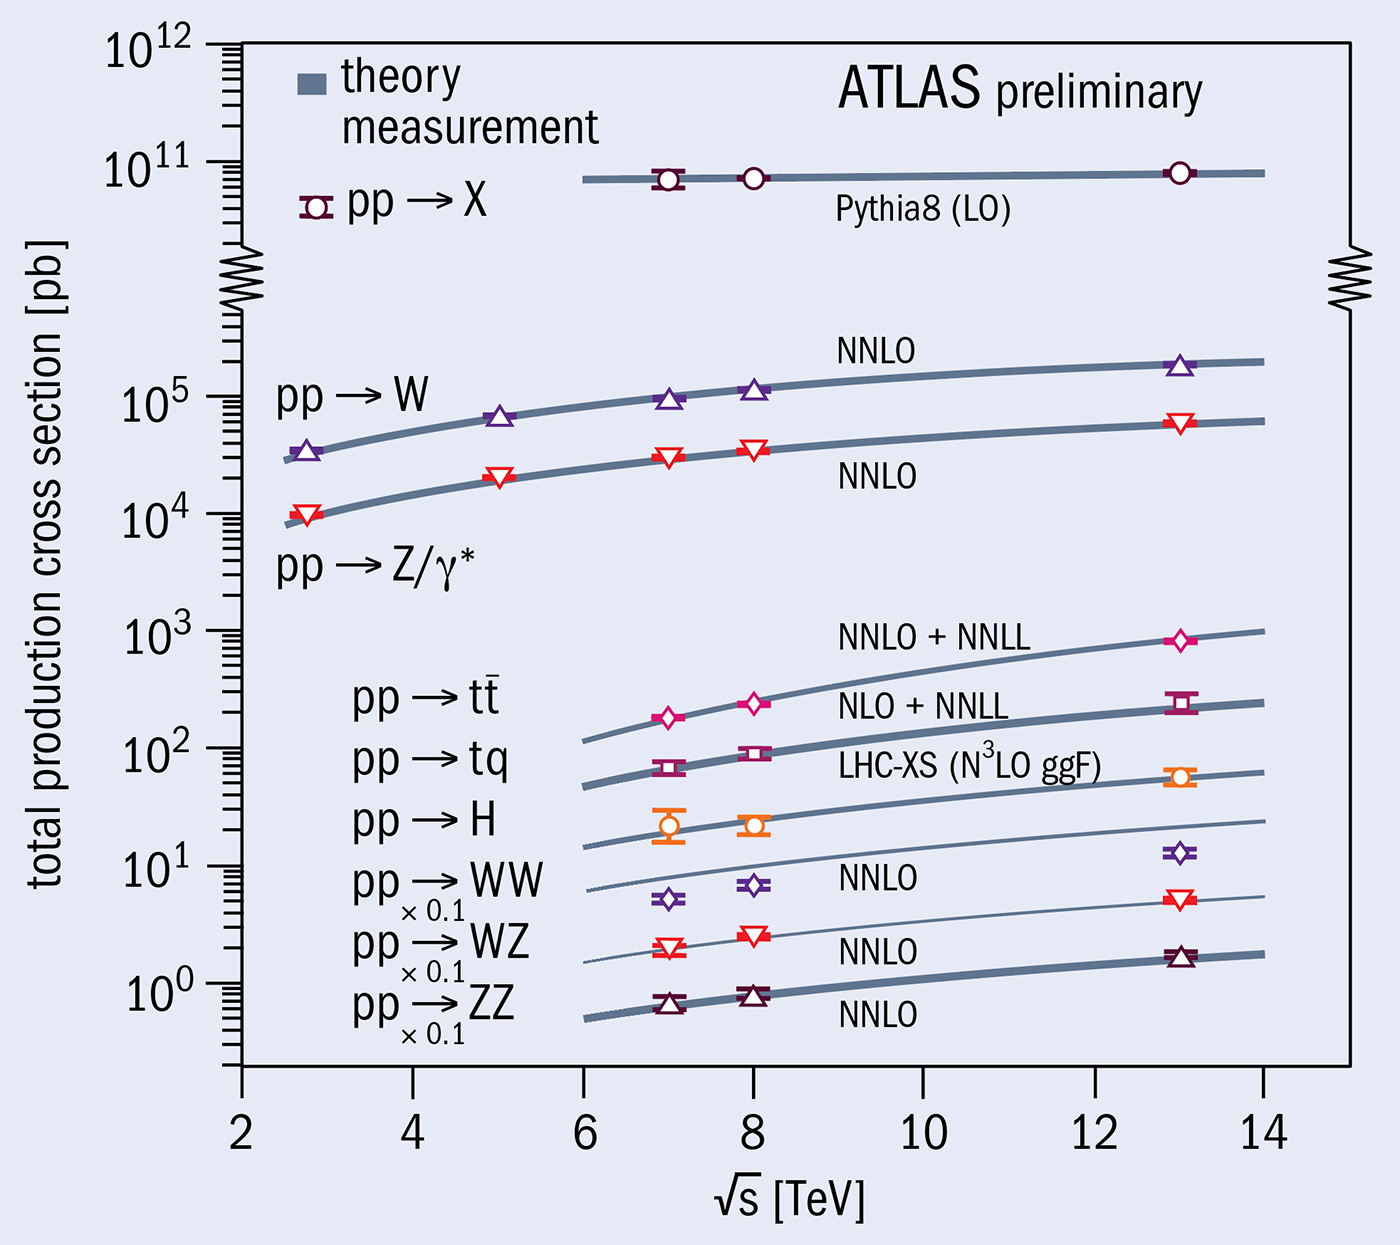
\includegraphics[scale=0.2]{gfx/ch5/CCMarApr_LHC10_fig2.jpg}\quad
    %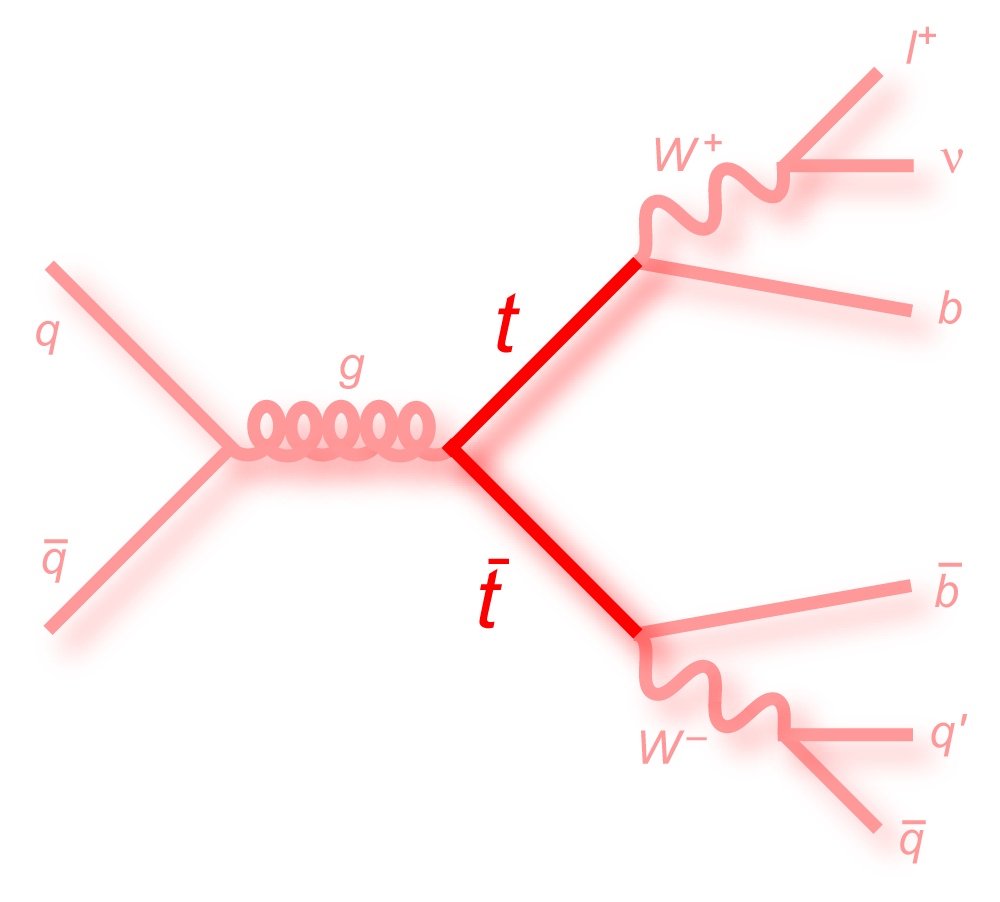
\includegraphics[scale=0.3]{gfx/ch5/feynman_ttbar_ljets_longt.png}
    %\caption[t$\overline{\text{t}}$ diagram]{ The t$\overline{\text{t}}$ process is dominating the cross sections at LHC, making it one of the leading SM background processes. Bottom: the production diagram for proce}
    %\label{fig:ttfig}
%\end{figure}

Having at our disposal a large set of FullSim MC NanoAOD samples for t$\overline{\text{t}}$ events, we used these to \emph{train} our models on the two target objects.

\subsection{Jets}

As discussed in Section \ref{sec:nanoaod}, a NanoAOD, i.e. the CMS standard analysis format, contains both the Jet objects, i.e. final-state reconstructed jets, and the GenJet objects, the jets resulting from the clustering of initial, Gen-level particles before going through the reconstruction step. The latter are either matched to Jet objects, or may end-up unmatched because of limitations in the matching algorithms and the previous simulation steps. For the moment, we disregard the problem of \emph{fake jets}, that is Jet objects which are not matched to a GenJet object but are instead due to noise or Pile-Up.

The idea is being able to directly generate correctly distributed Jet objects starting from noise, for stochasticity,  but also from the values of a corresponding GenJet, as a physical-informed input for the network (a process known as \emph{conditioning}): knowing just the generator-level information of some process, we are going to skip the Simulation, Digitization and Reconstruction steps.


With the use of \texttt{C/C++} code for the \texttt{ROOT} data analysis framework \cite{Brun:491486}, we processed the NanoAOD files and extracted all the Jet objects matched to a GenJet object, across all the events in the file. Because of the large number of variables, we selected a meaningful subset, containing all the necessary information for our test analysis.

First of all, we selected the following 14 GenJet variables for conditioning the generation: 

\begin{outline}
\1 \emph{The physical properties} of the GenJet, that is $\eta$, $\phi$, $m_j$, $p_T$, and the \emph{Parton} and \emph{Hadron Flavour}, giving the \emph{flavour} content of a jet as containg a specific quark or some gluons;

\1 \emph{Variables correlated with the rest of the event}, as the actual properties of a jet are expected to be influenced by other objects such as muons. Computing the $\Delta$R separation between the GenJet and the GenMuons present in the event, we selected the first and second \emph{closest muons}, and we computed the following quantities for each one:
\2 \texttt{Dr}, giving the separation from the GenJet, \texttt{DEta}, the $\eta$ difference from the GenJet, \texttt{DPt}, the $p_T$ difference from the GenJet, \texttt{DPhi}, the $\phi$ difference from the GenJet;

\1 If no GenMuons were present within a cone of $\Delta$R = 0.5 from the GenJet, the corresponding values were set to a user-defined maximum.

\end{outline}

Then, we selected the following 17 target reconstructed variables for the matched reconstructed Jet objects:

\begin{outline}
\1 \emph{The physical properties} of the Jet \emph{with regard to} the ones of the matched GenJet: $\Delta\eta$, the $\eta_{reco} - \eta_{gen}$ difference , $\Delta\phi$, the $\phi$ difference, $R_m$, the ratio of the jet and GenJet masses, $R_{p_T}$, the ratio of $p_T$s. This was done because the Simulation and Reconstruction steps are expected to introduce corrections w.r.t. the GenJet distributions, easier to learn when considering these quantities. As an additional variable, the Jet \texttt{Area}, a measure of its susceptibility to radiation, like pileup or underlying event, was added as well;

\1 Some of the btag discriminant variables \emph{b-tagging and c-tagging algorithms scores}: \texttt{btagCMVA}, \texttt{btagCSVV2}, \texttt{btagDeepB}, \texttt{btagDeepC}, \texttt{btagDeepFlavB} and \\\texttt{btagDeepFlavC}, which indicate with a score ranging from 0 to 1 whether the Jet contains the respective quark or not, a very significant information for performing event selection during an analysis. Some values may be offsetted to -1 to indicate that the corresponding tagging algorithm has faild to assign a score to the event;

\1 The \texttt{bRegCorr}, the $p_T$ correction for b-jet energy regression, as the presence of neurinos due to semi-leptonic decays in the jets coming from b quarks can result in underestimated jet energy measurements;

\1 The \texttt{qgl} score for the Quark vs Gluon likelihood discriminator, which is employed as most of the interesting physics channels studied at the LHC involve hadronic jets initiated by quarks, while dominant backgrounds often arise from QCD events, where jets are generally produced from gluons;

\1 The \texttt{jetID} and \texttt{puID} ID flags indicating relevant characteristics of the jet as well as the event noise and Pile-Up.
\end{outline}
\subsection{Muons}

For muons we performed the same procedure, taking only those muons matching to GenMuon objects (a GenParticle object with pdgId value of $\pm$13). 

We selected 30 GenMuon variables for conditioning:

\begin{outline}
\1 \emph{The physical properties} of the GenMuon, that is $\eta$, $\emph{phi}$, \texttt{Charge} and $p_T$;

\1 \emph{The 14 GenParticle status flags}, a series of \texttt{statusFlags} stored bitwise, with each bit having a different physical interpretation such as \emph{isTauDecayProduct}, \emph{fromHardProcess}, etc. or some information regarding the position of the object in the detector;

\1 \emph{Variables correlated with the rest of the event}, as the actual properties of a muon are expected to be influenced by other objects such as jets. Computing the $\Delta$R separation between the GenMuon and the GenJets present in the event, we selected the first \emph{closest GenJet}, and we computed the following quantities:
\2 $\Delta$R, giving the separation from the GenJet, $\Delta\eta$, the $\eta_{muon} - \eta_{jet}$ difference, $R_{p_T}$, the ratio of $p_T$s, $\Delta\phi$, the $\phi$ difference, and finally the $m_j$ of the closest GenJet;

\1 A series of 6 \emph{ Event level variables regarding Pile-Up}:\\ \texttt{Pileup\_gpudensity}, the Generator-level PU vertices/mm,\\ \texttt{Pileup\_nPU}, the number of pileup interactions that have been added to the event in the current bunch crossing, \texttt{Pileup\_nTrueInt}, the true mean number of the poisson distribution for this event from which the number of interactions each bunch crossing has been sampled, \texttt{Pileup\_pudensity}, PU vertices/mm, \texttt{Pileup\_sumEOOT}, the number of early out of time pileup and \texttt{Pileup\_sumLOOT}, the number of late out of time pileup;
\end{outline}

Then we selected 22 target variables for the Muon objects:

\begin{outline}
\1 \emph{The physical properties} of the muon \emph{with regard to} the ones of the matched GenMuon: \texttt{EtaMinusGen}, the $\eta$ difference , \texttt{PhiMinusGen}, the $\phi$ difference, \texttt{PtRatio}, the ratio of $p_T$s. This was done because the Simulation and Reconstruction steps are expected to introduce corrections w.r.t. the GenMuon distributions, easier to learn when considering these quantities. As an additional variable, the \texttt{ptErr}, the $p_T$ error for the muon track, was selected as well;

\1 Six \emph{impact parameters} with respect to the primary vertex: \texttt{dxy}, \texttt{dxyErr}, \texttt{dz}, \texttt{dzErr}, the 3D impact parameter \texttt{ip3d} and its significance \texttt{sip3d}, all expressed in cm;

\1 Some \emph{Boolean flags}: \texttt{isGlobal}, \texttt{isPFcand}, identifying the muon as a Particle Flow candidate, \texttt{isTracker};

\1 A series of \emph{isolation variables} returned by the Particle Flow algorithm: \texttt{pfRelIso03\_all}, \texttt{pfRelIso03\_chg} and \texttt{pfRelIso04\_all};

\1 The \emph{variables related to the closest jet}: \texttt{jetPtRelv2}, indicating the relative momentum of the lepton with respect to the closest jet after subtracting the lepton and \texttt{jetRelIso}, the relative isolation in matched jet;

\1 A series of \emph{ID scores}: \texttt{mediumID}, \texttt{softMVA} score and its cut-based ID \texttt{softMVAId}, \texttt{softId};
\end{outline}

\subsection{Extraction and preprocessing}

We processed the NanoAOD files and extracted all the Jet objects matched to a GenJet object and the Muon objects matched to a GenMuon across all the events in the file.
The output of the \emph{extraction} step is another \texttt{.root} file containing just the selected objects.

The resulting file is still organized according to the Events structure. Besides, we know that many machine learning algorithms work best when specific distributions are \emph{preprocessed} according to specifc criteria. Normalizing Flows are no exception. Specifically, there are four key features which should be accounted for and modified through preprocessing before training:

\begin{figure}
    \centering
    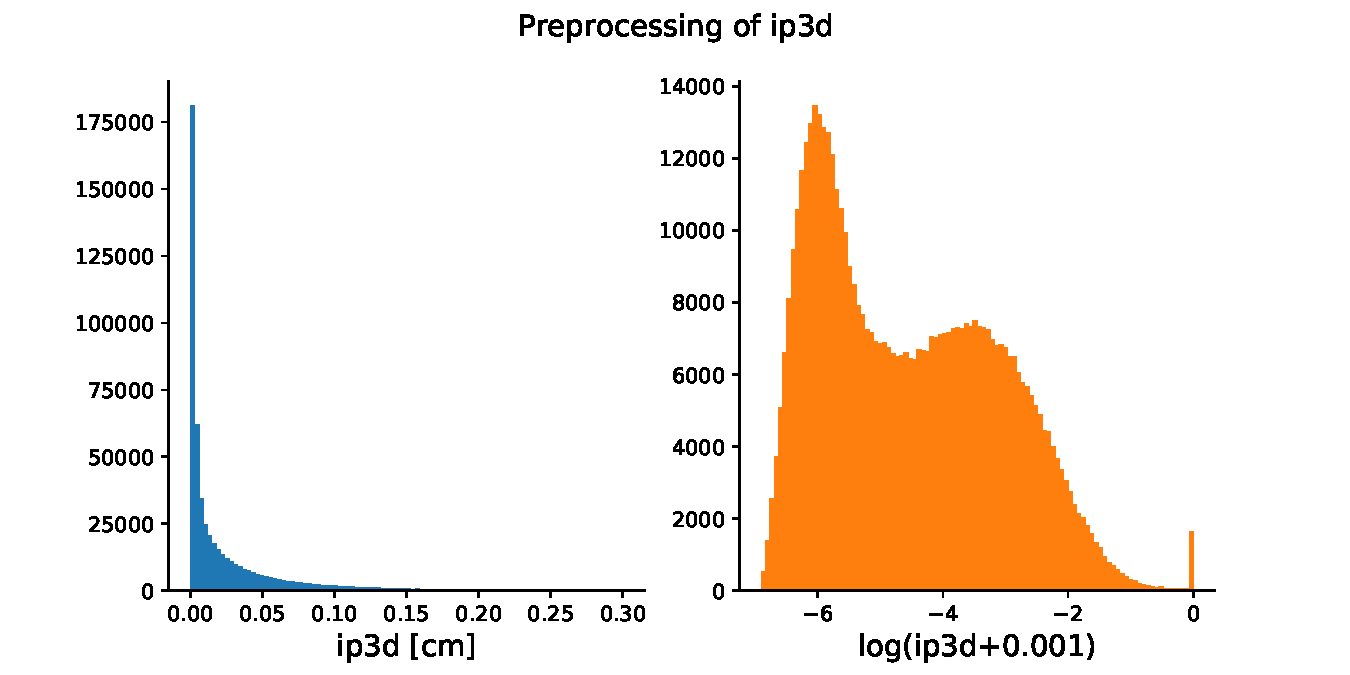
\includegraphics[width=\columnwidth]{gfx/ch5/preproce.pdf}
    \caption[Preprocessing]{Sharply peaked distribution are being converted to more broad ones during the preprocessing step. In this example the \texttt{ip3d} variable gets transformed as log(\texttt{ip3d}+0.001).}
    \label{fig:preproce}
\end{figure}

\begin{outline}
\1 Because NF are learning actual pdfs, \emph{large gaps} between values of the distribution may disturb training and trick the network to \emph{bridge} the extremes of the distribution by creating spurious samples in the gap. When possible, the gaps should be reduced and the values packed closer together;

\1 As NF assume a continuous and differentiable pdf, they are not well suited to deal with \emph{discrete} distributions. Thus, we should apply a process known as \emph{dequantization}, that is applying some sort of smearing to the discrete values to make them similar to those sampled from a continuous distribution;

\1 For similar resons as before, when possible it would be beneficial to widen and normalize sharply peaked distributions through invertible transforms such as log(x). If well separated, eventual peaks may be dequantized as well;

\1 Finally, we opted for \emph{saturating} long tails of distributions to some limiting values, in order to make it easier for the model to learn the pdf in the more populated region.
\end{outline}

Apart from possibly dequantization, we stress that all of this transformations were implemented to make training easier but are not strictly necessary--the models revealed themselves as powerful enough to deal with complex, sharply peaked, long tailed distributions. However, having already implemented the preprocessing pipeline and because it did not introduce a big overhead in the procedure, we decided to keep it for the present work. An example of one of the possible preprocessing operations is shown in Figure \ref{fig:preproce}.

All of these transforms may be implemented with a clear and natural syntax in the \texttt{Python} programming language, specifically thanks to the \texttt{pandas} package \cite{reback2020pandas}, which implements a convenient dataframe structure.

\section{Models design}
This section describes the implementation  details for the two architectures--the one responsible for the generation of jets and the one targeting muons. We discuss the software choices and then the model specifics and trainings.

\subsection{Software and packages}

We initially planned to use another class of generative models, that is Generative Adversarial Networks. However, after discovering the work of Dr. Stephen Green \cite{stephen_green_2021_4558988} we realized that Normalizing Flows were better suited to our task, as they suffered from less training instabilities and allowed us to directly learn the underlying distributions with an easily interpretable loss function.

The models are implemented following Dr. Green's example: the \texttt{Python} package \texttt{nflows} \cite{conor_durkan_2020_4296287} defines the Classes for Rational Quadratic Spline Normalizing Flows, integrating them for use with the popular ML research package \texttt{Pytorch} \cite{NEURIPS2019_9015}. We optimized the hyperparameters choices for our use case as best as possible, a process resulting in the architectures presented below.

\subsection{Architectures and trainings}

\begin{figure}
    \centering
    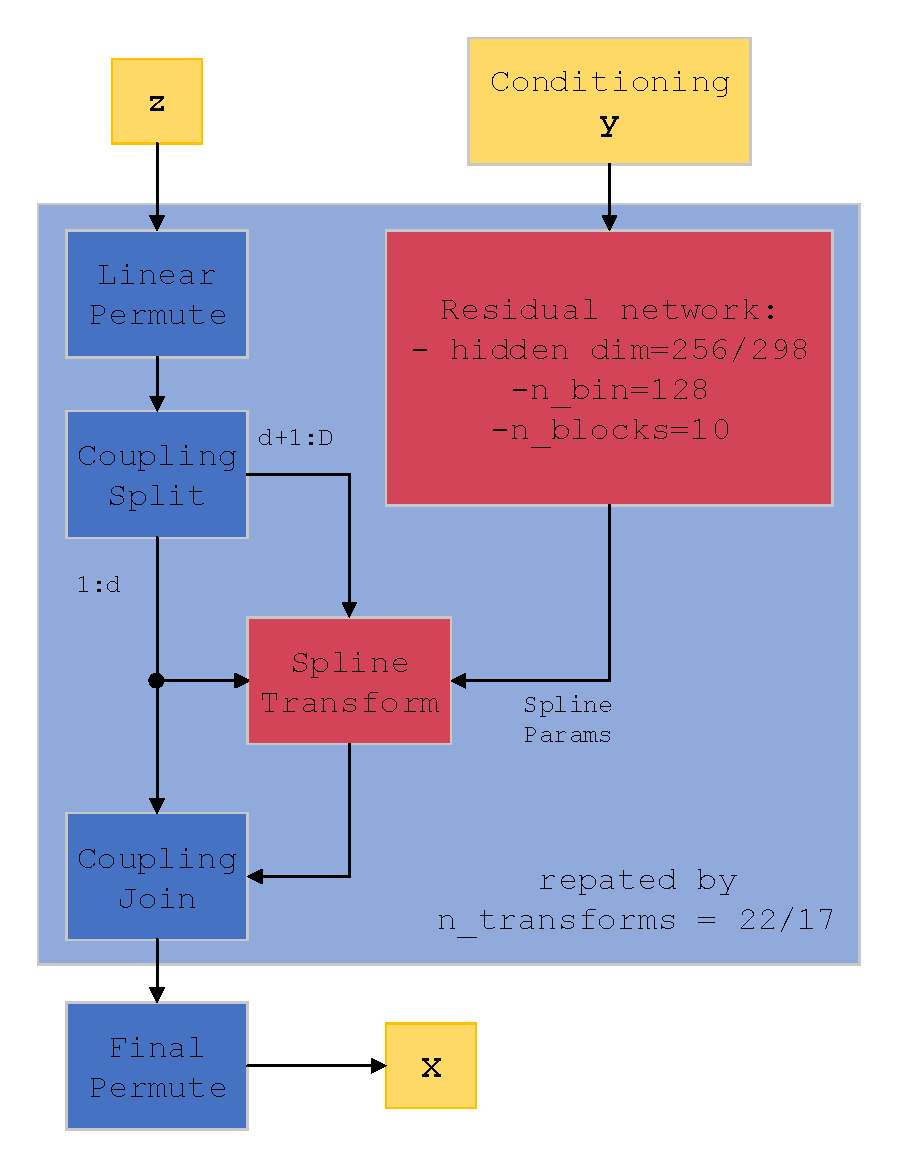
\includegraphics[width=\columnwidth]{gfx/ch5/nfmodel.pdf}
    \caption[Actual NF model]{The NF models are quite large and complex. A number of transforms equal to that of the target variables is performed. The normally distributed inputs \textbf{z} are permuted for each step and then splitted in half, sending half as parameters and half as argument of the \emph{spline transform}. The conditioning variables \textbf{y} are sent as input to a complex 10 layer residual network (different for each transform) which defines the parameters for the spline. Everithing is repeated until the last step where we permute back to the original order and output the targets \textbf{x}. Where two numbers are separetad by a slash, the first refers to the muons model, the second to the jets one.}
    \label{fig:nfmodel}
\end{figure}

Figure \ref{fig:nfmodel} shows the final models employed in this work. 
As discussed in Section \ref{sec:couplay}, in order to reduce the computational complexity of the Jacobian in the NF loss function, we implemented the total transformation as a chain of single, subsequent splines transformations, each acting on just half of the input, while the latter half is kept unchanged and serves as additional parameters for the splines. This has the additional advantage of ensuring good \emph{correlations} between the various variables, as the transformation for one of them will end up depending on every other variable as long as we implement a number of transformation equal to the number of variables and we permute the order linearly before each spline.

For each spline, the normally distributed inputs \textbf{z} are permuted and then splitted in half, sending half as parameters and half as argument of the \emph{spline transform}. The conditioning Gen-level variables \textbf{y} are sent as input to a complex 10 layer fully-connected \emph{residual} network (a different one for each transform) which defines the parameters for the spline. Its most relevant hyperparameters are the \emph{hidden\_dim}, the number of nodes per hidden layer, set to 256 for the muons model and to 298 for the jets one, the \emph{n\_bin}, the number of bins for the spline, set to 128 for both models and the \emph{n\_blocks} set to 10 for both and defining the number of hidden layers.
Each network was defined with \texttt{ReLU} activation function and setting \texttt{batch\_norm=True}. The training procedure actually traverse the network in the opposite way, strarting from the training data and using the inverse transform to obtain normally distributed instances which can easily be evaluated in the NF loss function.

We would like to emphasize the fact that because \emph{each transform} defines a separate network for learning the optimal spline parameters, the final models are quite large, especially for physics-based application standards. The muons model exceeds 54e6 trainable parameters (54,988,164 parameters, corresponding to the various weights of the neurons in each layer and the batch norm parameters), while the jets model totals in at 47,986,595 parameters. These large models were trained on around 5e6 muons or jets objects extracted as explained above, and the \emph{losses} were monitored at each epoch on a separate \emph{validation set} of about 4e5 samples to ensure that the models were not being over-optimized for the training set. Additionally, we saved the model state every 10 epochs and performed additional validation on a separate set of $10^5$ data to further avoid overfitting.

As our \emph{optimizer} algorithm we choose the de-facto standard in the field, the \texttt{Adam} algorithm \cite{https://doi.org/10.48550/arxiv.1412.6980}, a complex and powerful algorithm for models optimization still based on the same basic principles of \emph{gradient descent} explained in Section \ref{sec:backprop}, with an initial \emph{learning rate} of $10^{-4}$ for muons and $10^{-5}$ for jets, reduced during training by the \emph{cosine annealing} procedure. The maximum epochs were set to 1000 for the muons model, giving its larger number of target variables, and to 500 for the jets one--this also means that the learning rate reduction due to cosine annealing will be different over training as it depends on the total epochs number.

Trainings were stopped respectively at epoch 580 for muons and at epoch 420 for jets, as we had reached a good convergence, despite both models showing signs for more improvements. Figure \ref{fig:losses} shows the models losses over the training epochs. The validation loss is plotted by averaging over the last 5 epochs, to display the overall trend instead of single, noisy variations. The values on the y-axis are the actual loss values, and they are obviously different as they depend on both the number and the ranges of the target variables.


\begin{figure}
    \myfloatalign
    \subfloat[]
    {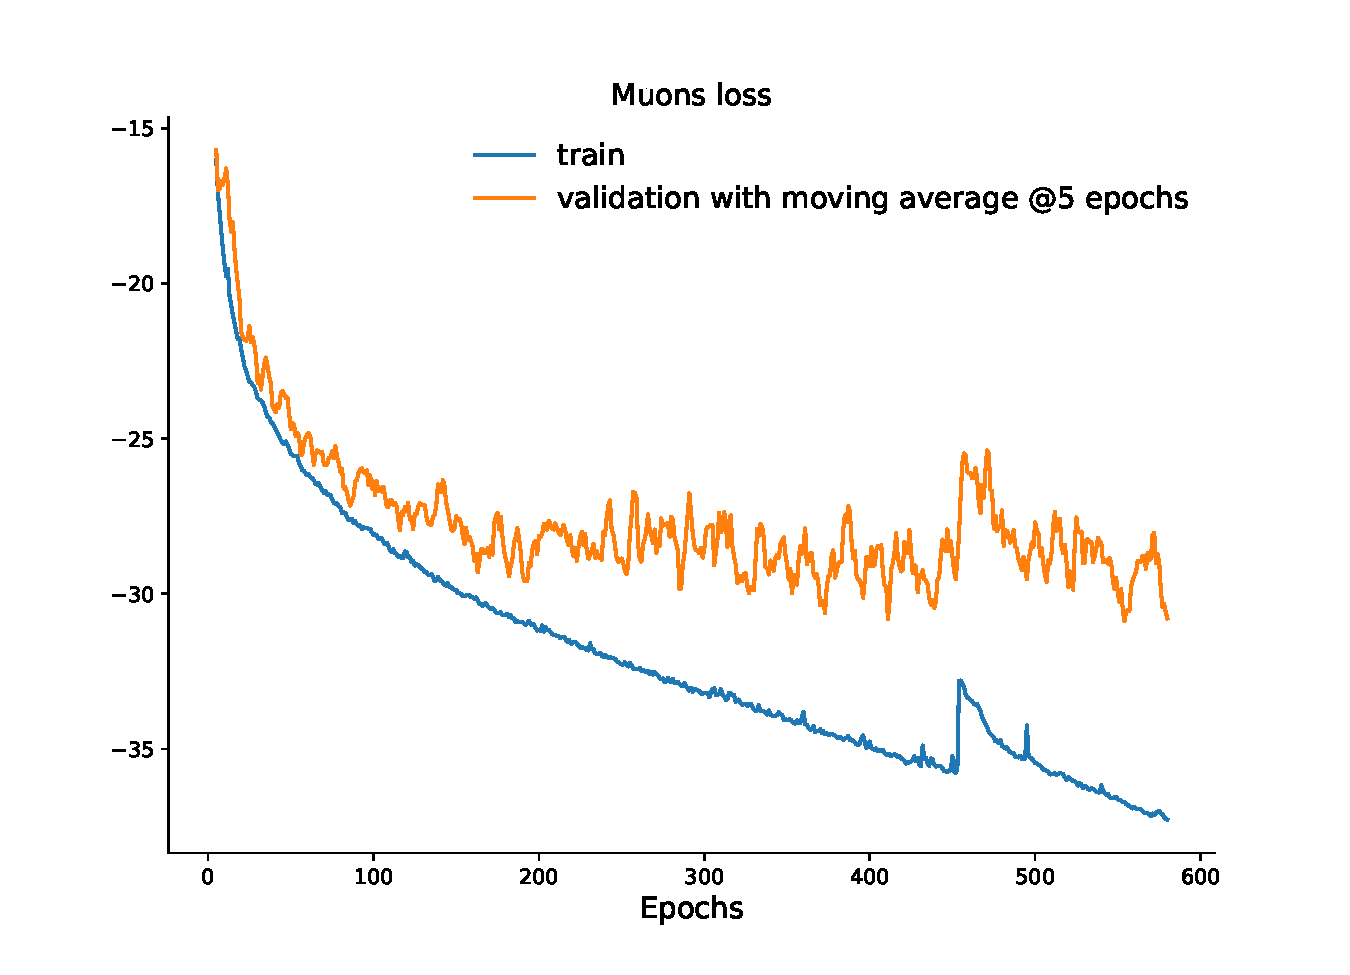
\includegraphics[width=\linewidth]{gfx/ch5/lossesmuons.pdf}} \\
    \subfloat[]
    { 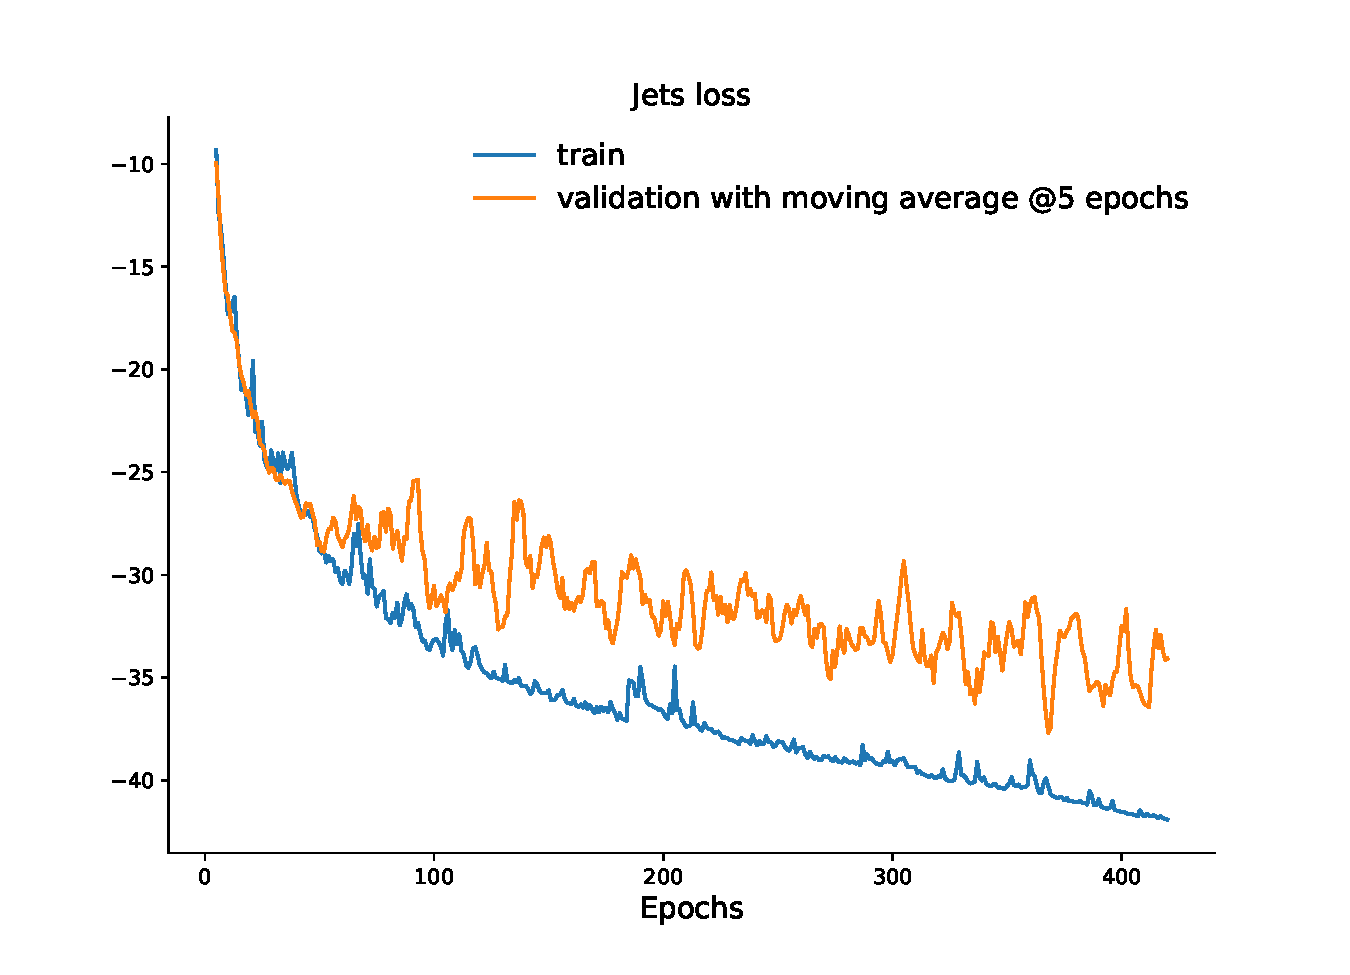
\includegraphics[width=\linewidth]{gfx/ch5/lossesjets.pdf}} 
    \caption[Models losses]{The training for both models (a muons and b jets) has reached a good convergence, but there is still room for improvements. The losses are plotted starting from epoch 5 to better display the decrease in the final epochs.}\label{fig:losses}
    
\end{figure}

We trained the models on the local INFN Pisa computing resources, specifically on a \texttt{NVIDIA V100} GPU with 32GB of VRAM and 5,120 CUDA Cores. The time spent for the training of both models was $\approx$ 5 days, however we observed that due to inefficient \emph{data loading} on the GPU, the maximum usage of the device fluctuated between 40$\%$ and 80$\%$ most of the time, indicating that more data loading resources or a different training scheme (such as \emph{distributed training}) could improve training times decisively.

\section{Results}

\graffito{do we want to plot the full results in an appendix?? or refer to a colab??}
We move on to discuss the results obtained. 
To perform a sound and reasonable comparison, we extract the Gen-values for conditioning from $10^{5}$ samples coming from an unseen test set for jets and from the validation set (which was not used for training but just for evaluating the loss over time) for muons. We then generate new FlashSim samples starting from the same Gen-values, to get a one-to-one correspondence between the two sample sets.
It has been observed that when generating a larger number of events, in the order of millions to billions, low probability mass regions can produce negative, nonphysical values. This phenomenon is very rare and can be easily corrected by implementing a check in the postprocessing, regenerating the event through the extraction of new noise values to sample from a different region of the learned pdf.

There are two main types of comparison which can now be performed on the obtained samples: we can compare the \emph{distribution} or the \emph{correlations} for the two.
While the latter can be inspected visually thanks to \emph{contour plots}, we would like to define a precise measure for the similarity of the empirical distributions between two samples. We thus define the \emph{Wasserstein distance} as:

\[W_1(u, v) = \inf_{\pi \in \Gamma(u, v)}\int_{\mathbb{R}\times\mathbb{R}}\abs{x-y}d\pi(x,y) = \int_{-\infty}^{+\infty} \abs{U - V}\]

where $\Gamma(u, v)$ is the set of (probability) distributions on $\mathbb{R}\times\mathbb{R}$ whose marginals are $u$ and $v$ on the first and second factors respectively, and $U$, $V$ are the respective CDFs. Intuitively, if each distribution is viewed as a unit amount of earth (soil), the metric is the minimum \emph{cost} of turning one pile into the other, which is assumed to be the amount of earth that needs to be moved times the mean distance it has to be moved, and thus this metric is also know informally as the \emph{earth mover distance}.

\subsection{1d distributions and correlations}


\paragraph{Jets}

We show in Figure \ref{fig:jetsdists} four 1-d distributions from the total of 17 target variables obtained for jets. We emphasize once more that the model actually learned to generate the 17 values simultaneously, preserving the correct correlations as well as producing convincing distribution.

Regarding the distributions, we observe that the model has correctly learned all the multi-modal, sharply peaked tagging distributions with Wasserstein scores of the order of $10^{-3}$, testifying good convergence. The log scale of \texttt{btagDeepB} actually shows an instance of \emph{bridging}, where a small set of values were generated between two separate peaks. Single-mode distributions such as \texttt{ptRatio} have been larned as well, as were the Ids thanks to dequantization. The \texttt{jetId} plot in log-scale actually shows that a small set of samples has been generated in the empty regions between values 0, 2 and 6 (the only admissible ones) but this is because the continuous output of the network has been rounded to the nearest integer. A more refined version of post-processing is expected to correct this behaviour.

Finally, we also observe a worse performance on two distributions: \texttt{bRegCorr}, a rather simple, skewed one-mode distribution which is expected to improve with further training (current Wasserstein distance is $\approx$ 0.02), and \texttt{nConstituents}, plotted at the bottom of \ref{fig:jetsdists}. The latter result is probably in stronger disagreement because the target actually consist of integer values--as we discussed before, the NF approach expects continuous distributions, and so the model performs bridging in an attempt to obtain a reasonable continuous distribution. However, it has been observed in previous training for similar architerctures that the model is actually capable of overcoming this limitation by brute force alone: if left in training for long enough it will eventually learn to reproduce the discrete peaks of the target.

\begin{figure}
    \myfloatalign
    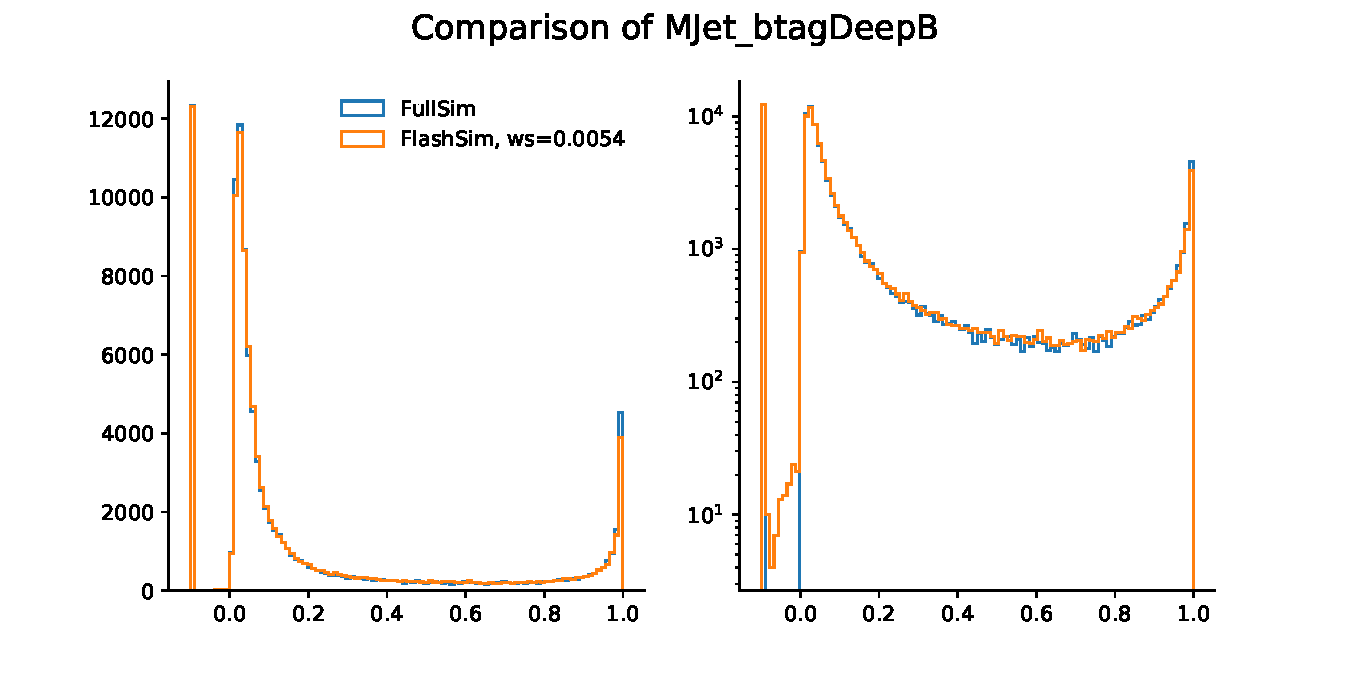
\includegraphics[width=\linewidth]{gfx/ch5/eval3.pdf} \\
    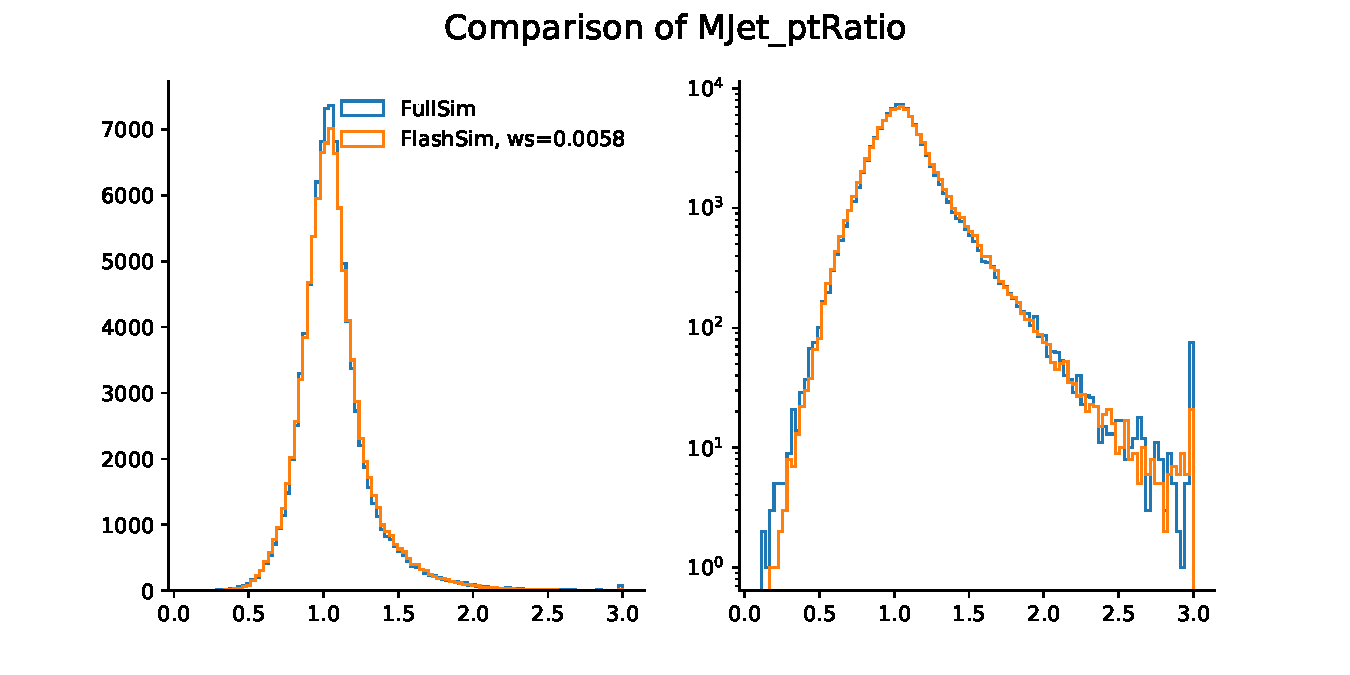
\includegraphics[width=\linewidth]{gfx/ch5/eval12.pdf} \\
    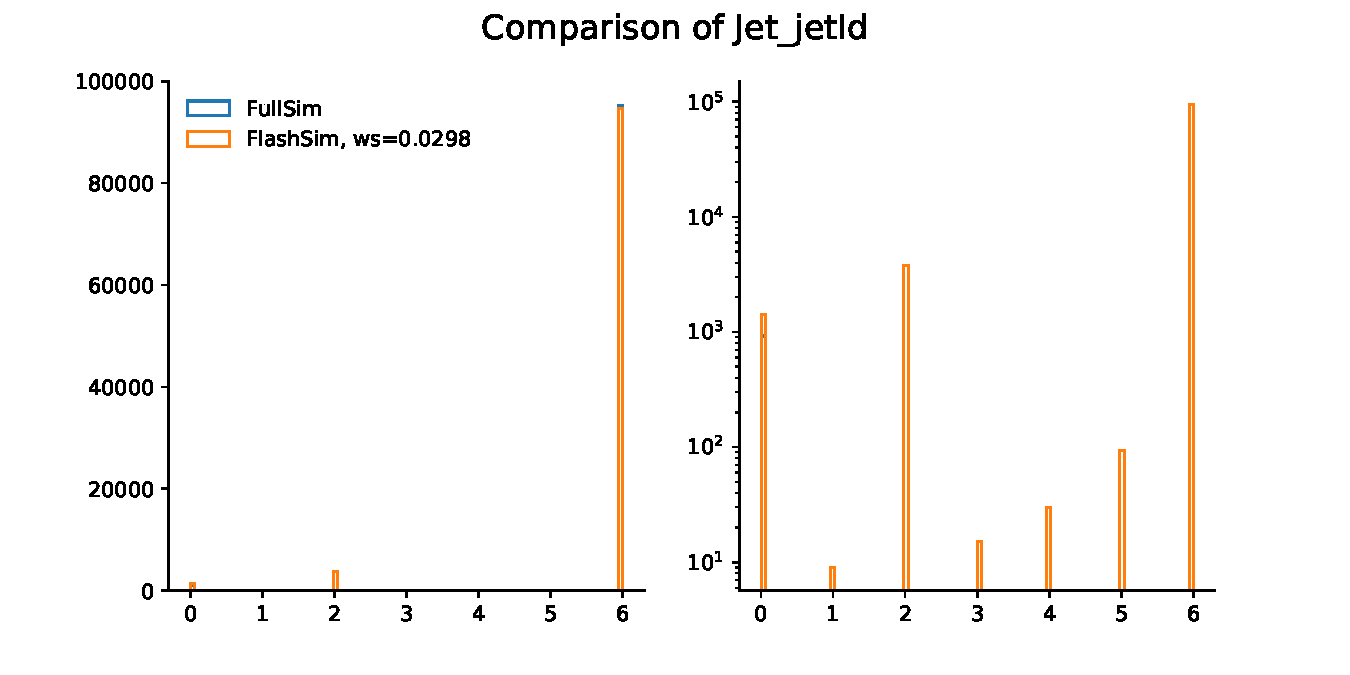
\includegraphics[width=\linewidth]{gfx/ch5/eval16.pdf} \\
    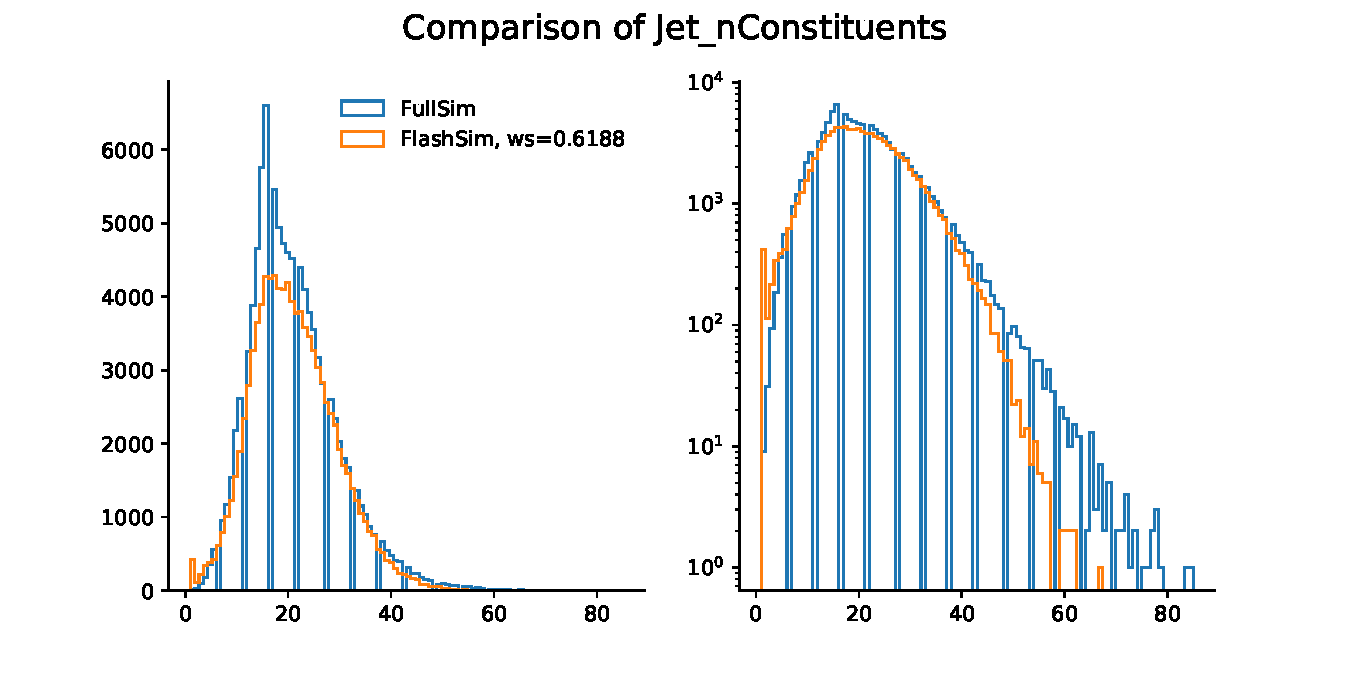
\includegraphics[width=\linewidth]{gfx/ch5/eval10.pdf}
    \caption[1-d jets distributions]{Four examples of 1-d distributions for jets. The model captures well multi-modal, sharply peaked distributions as well as single-mode, heavy tailed ones, and can also approximate Ids well thanks to dequantization. As expected it struggles with integers values such as \texttt{nConstituents}.}\label{fig:jetsdists}
    
\end{figure}

The correlations between jets variables, inspected visually, show good agreement with those from FullSim. Figure \ref{fig:corrjet1} shows the highly non-trivial correlations between the tagging distributions, with \emph{quantiles} plotted at 0.5, 0.9, 0.99. The same choice for quantiles has been adopted for all the following figures.

\begin{figure}
    \centering
    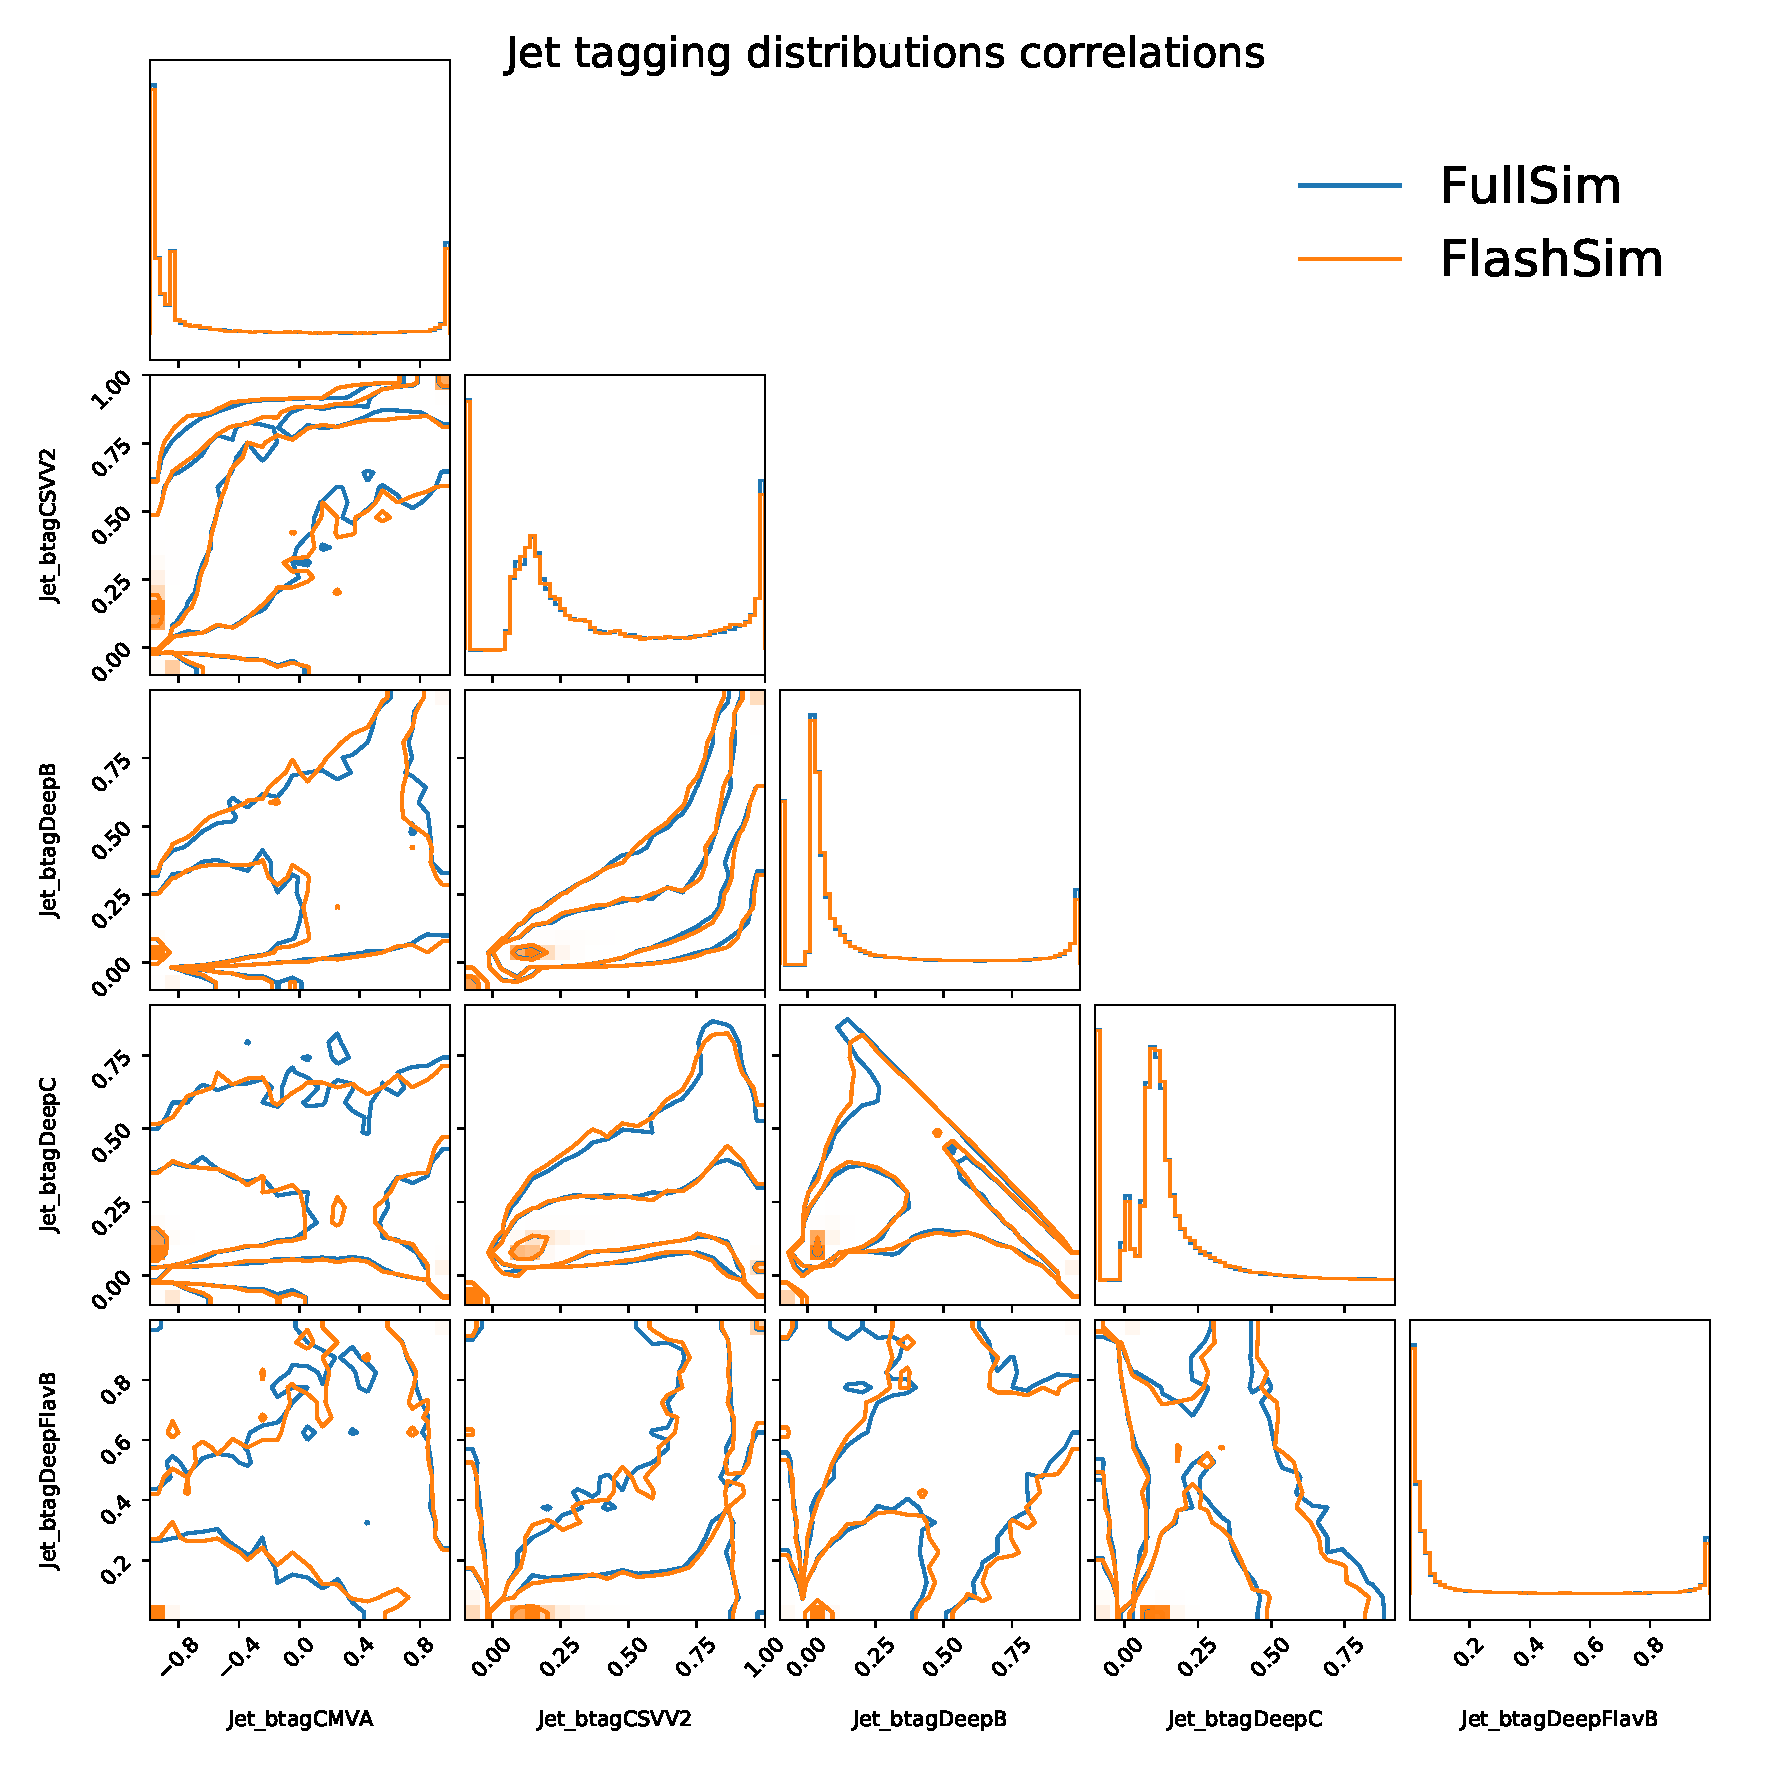
\includegraphics[width=\linewidth]{gfx/ch5/corrjet1.pdf}
    \caption[Tagging correlations]{Even non-trivial correlation such as the ones between tagging distributions are captured correctly by our models.}
    \label{fig:corrjet1}
\end{figure}

\graffito{get qgl nconstituens corr straight}
We can also observe in Figure \ref{fig:corrjet2+3} how the models have learned to capture the correlations between the qgl score, which is correctly correlated to the number of constituents as a lower number of constituents is expected for the u, d, s quarks when compared to gluons. Additionally, correlations between the physical p$_T$ and mass distributions, obtained from the original p$_T$Ratio and massRatio outputs of the network, are learned as well.

\begin{figure}
    \myfloatalign
    \subfloat[]
    {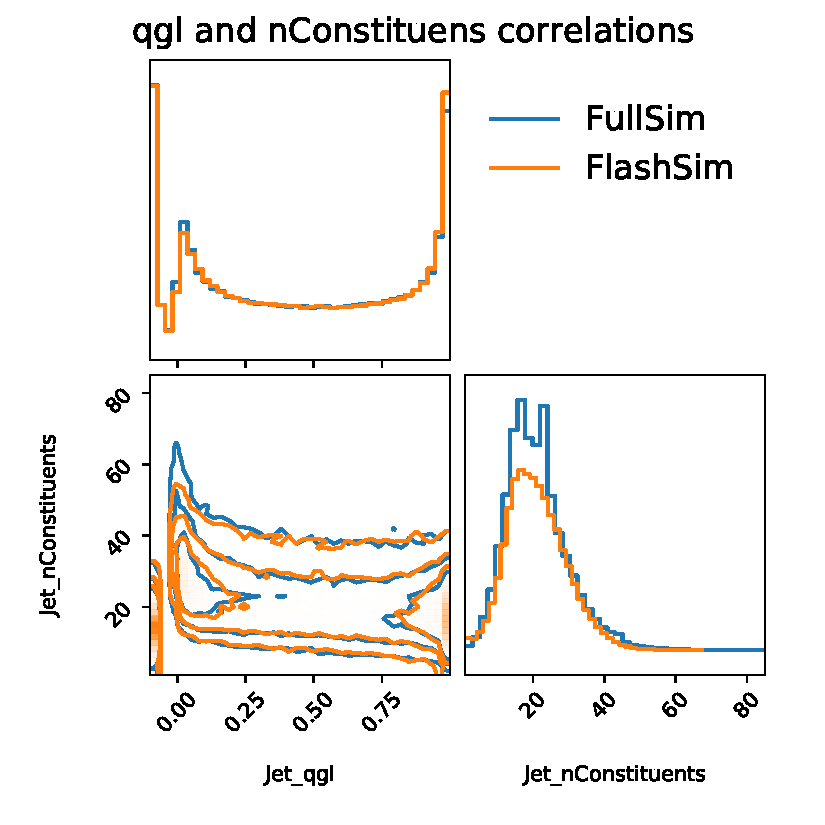
\includegraphics[width=0.45\linewidth]{gfx/ch5/corrjet2.pdf}}
    \subfloat[]
    { 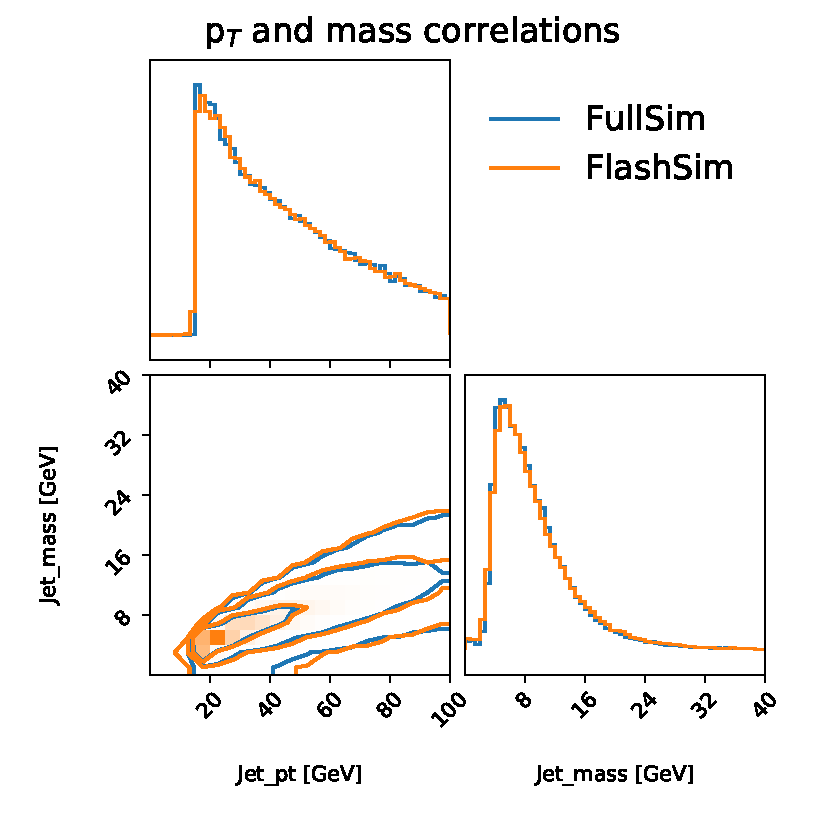
\includegraphics[width=0.45\linewidth]{gfx/ch5/corrjet3.pdf}} 
    \caption[qgl and p$_T$ correlations]{ (a) As expected, the qgl is positively correlated to the number of constituents--the lower the number, the larger the score. This behaviour has been captured by Flash Sim as well. The FullSim nConstituens distribution is jagged because of its discrete values, while the FlashSim has \emph{bridged} them and is thus smoothed.(b) The correlations between the physical distributions of p$_T$ and mass show agreement as well.}\label{fig:corrjet2+3}
    
\end{figure}

\paragraph{Muons}

For the muons, we obtained similar results--good, convincing general convergence and correlations apart from a subset of the target variable. It should be noted that a larger number of target variables for this case were actually Boolean Ids, and as discussed before were approached through dequantization. Figure \ref{fig:muonsdists} shows 4 distributions out of 22 target variables. Aside from good convergence on the firs two, we can observe that for a series of them, such as \texttt{dxyErr} and \texttt{dzErr} the training is complicated by the fact that the NanoAOD format stores the variables in a low-precision format: this is reflected by the jagged structure in the plot for FullSim and it causes the model to perform bridging to reach convergence.

\begin{figure}
    \myfloatalign
    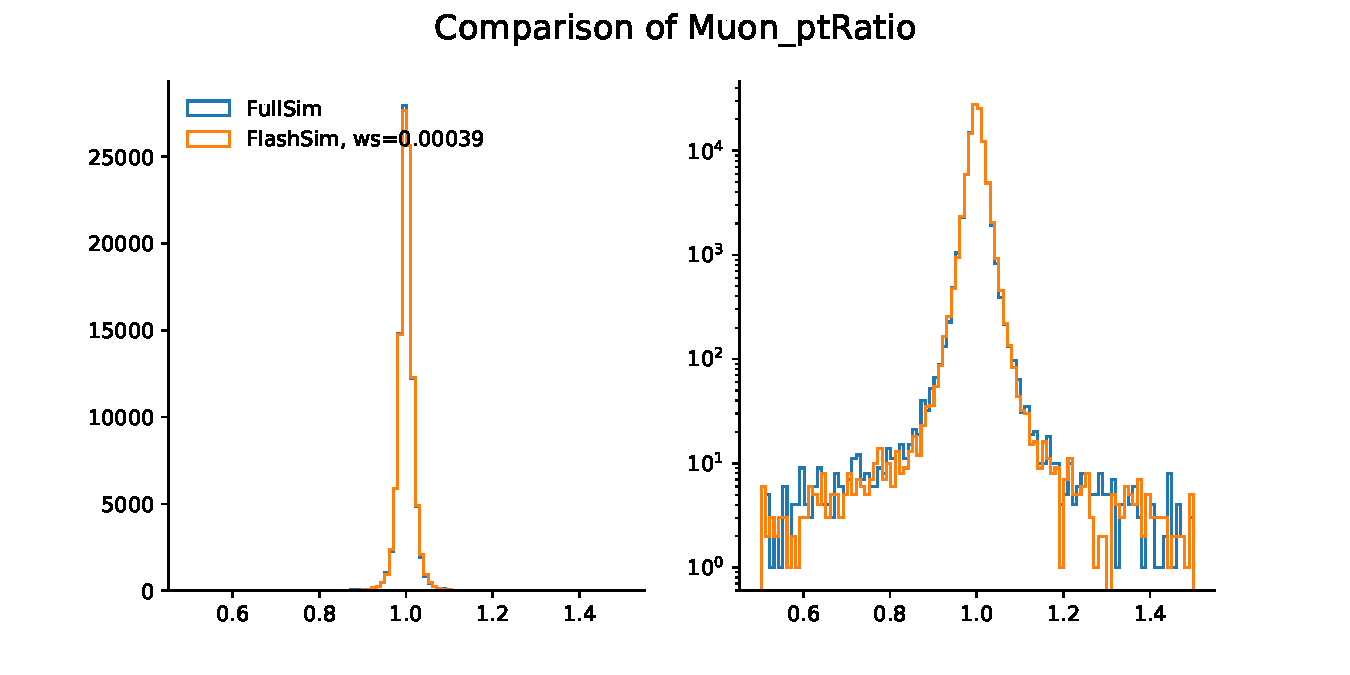
\includegraphics[width=\linewidth]{gfx/ch5/meval2.pdf} \\
    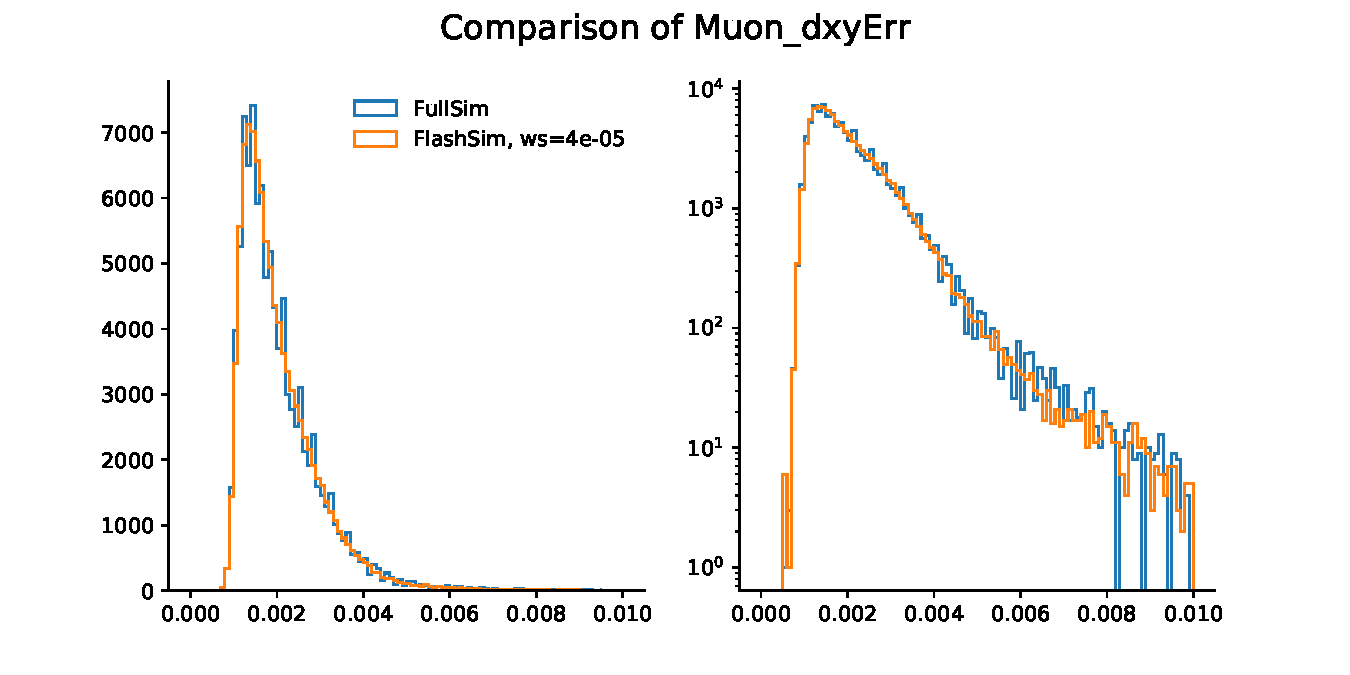
\includegraphics[width=\linewidth]{gfx/ch5/meval4.pdf} \\
    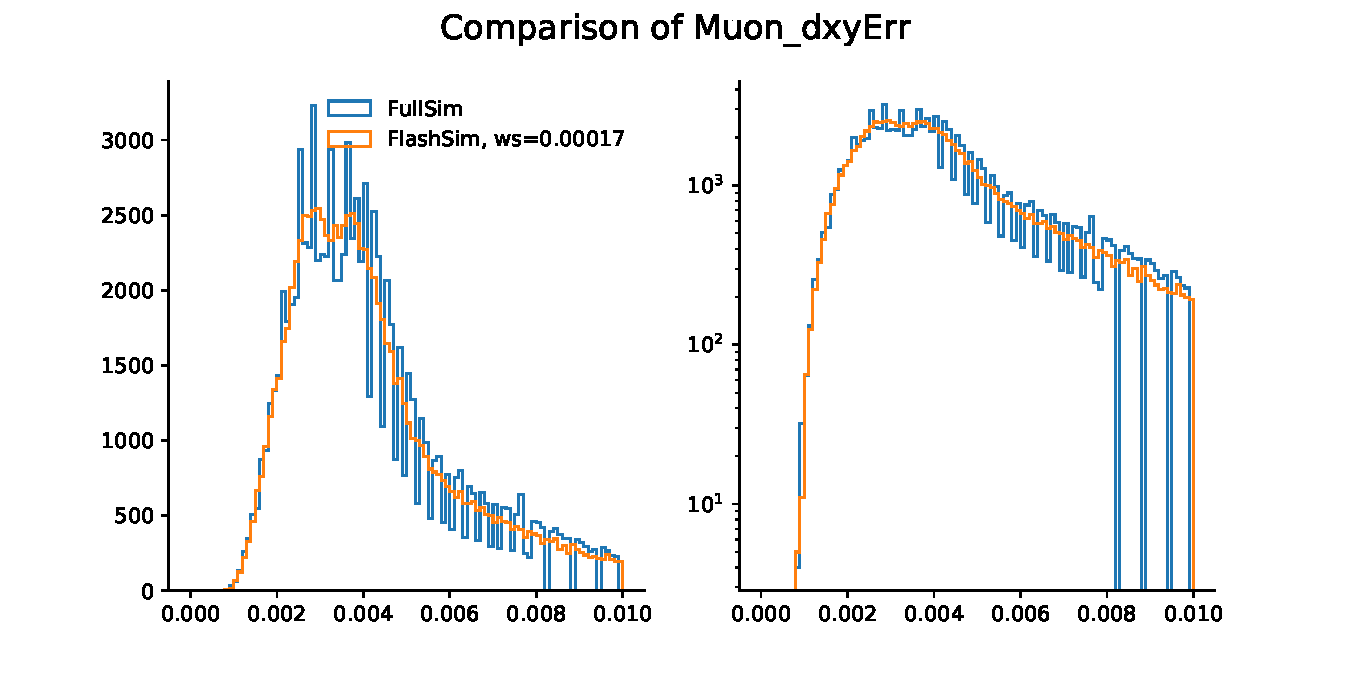
\includegraphics[width=\linewidth]{gfx/ch5/meval6.pdf} \\
    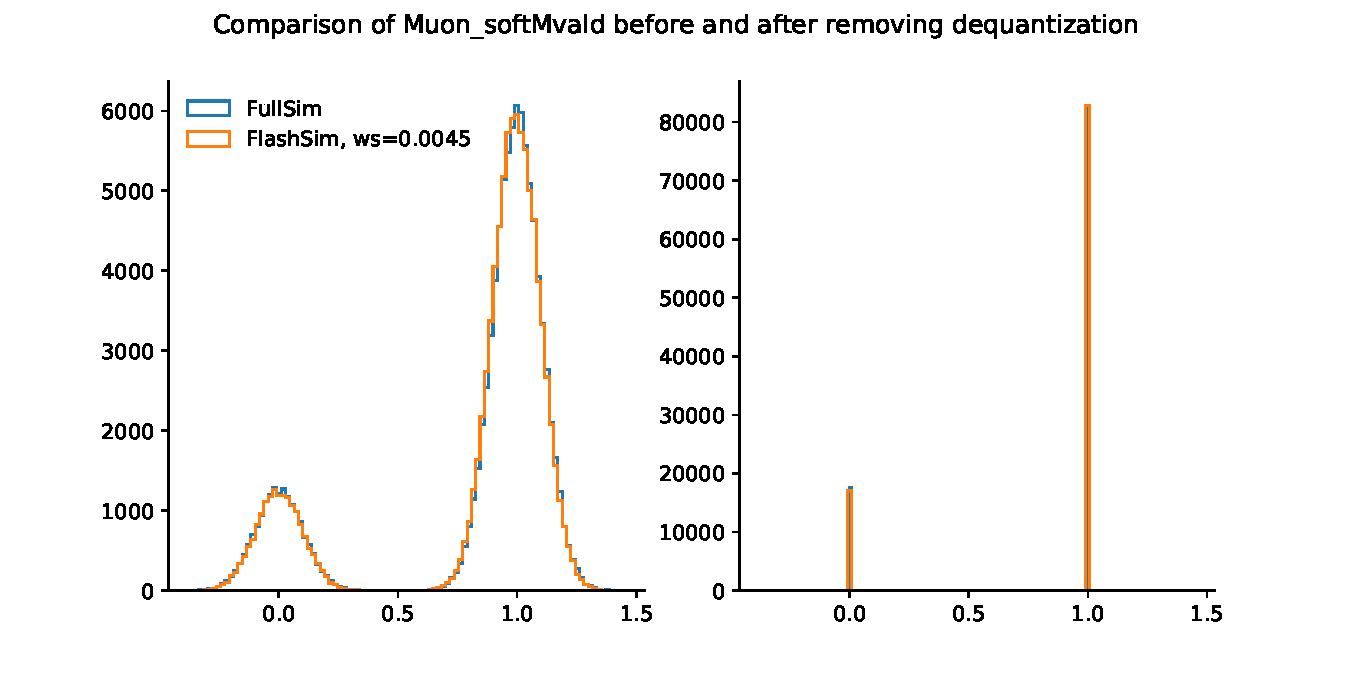
\includegraphics[width=\linewidth]{gfx/ch5/meval21.pdf}
    \caption[1-d muons distributions]{Four examples of 1-d distributions for muons. For most distributions the results present a small Wasserstein distance, however the model performs bridging in the presence of low-precision variables which present discrete peaks in the original FullSim..}\label{fig:muonsdists}
    
\end{figure}

\graffito{which is the exact relationship between ip3d and the sqrt?}
Finally, as a last example of correlations, we show in Figure \ref{fig:corrmuons} that the model has actually learned to capture complex correlations such as the ones between the \emph{impact parameter} \texttt{ip3d} and the quantity $\sqrt{\texttt{dxy}^2 + \texttt{dz}^2}$, which is closely related to the definition of the impact parameter itself.

\begin{figure}
    \centering
    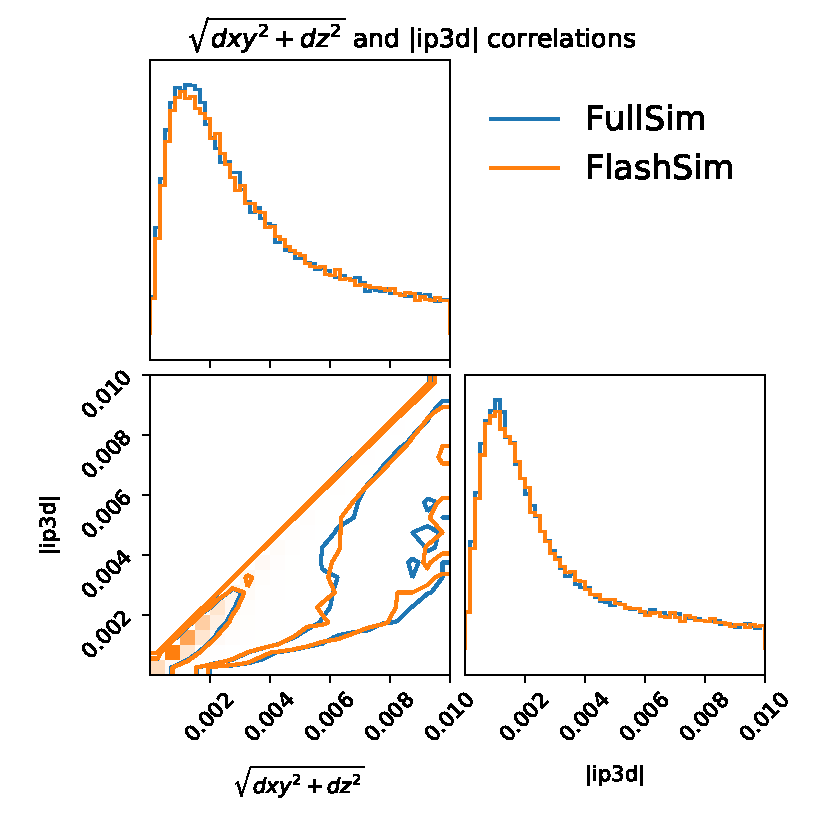
\includegraphics[scale=0.6]{gfx/ch5/mcorrs.pdf}
    \caption[Muons correlations]{The complex correlations between the \emph{impact parameters} \texttt{ip3d} and the related quantity $\sqrt{\texttt{dxy}^2 + \texttt{dz}^2}$ have been captured as well.}
    \label{fig:corrmuons}
\end{figure}


\subsection{Conditioning}

Another extremely important feature of our approach is the desired ability to obtain specific results starting from certain Gen-level inputs, a characteristic we called conditioning. 

We can readily see that this is possible by focusing on specific results obtained for the jets model. Figure \ref{fig:condit} shows that the final, NanoAOD level reconstructed p$_T$ is correctly correlated to the GenJet p$_T$ for both FullSim and FlashSim: as we would expect the Gen-p$_T$ is crucial in determining the final-state p$_T$. What is more, in the same figure we also show the \emph{profile histogram} and RMS ($\sigma_{p_T}$/p$_T$) for the GenJet p$_T$ versus the p$_T$Ratio. As expected, not only does the p$_T$Ratio decrease as the GenJet p$_T$ increases (highly energetic jets have a reconstructed p$_T$ closer to the Gen-value), but the RMS correctly decreases as well, as constant terms in the p$_T$ resolution due to PileUp are divided by bigger terms as GenJet p$_T$ increases.

\begin{figure}
    \myfloatalign
    \subfloat[]
    {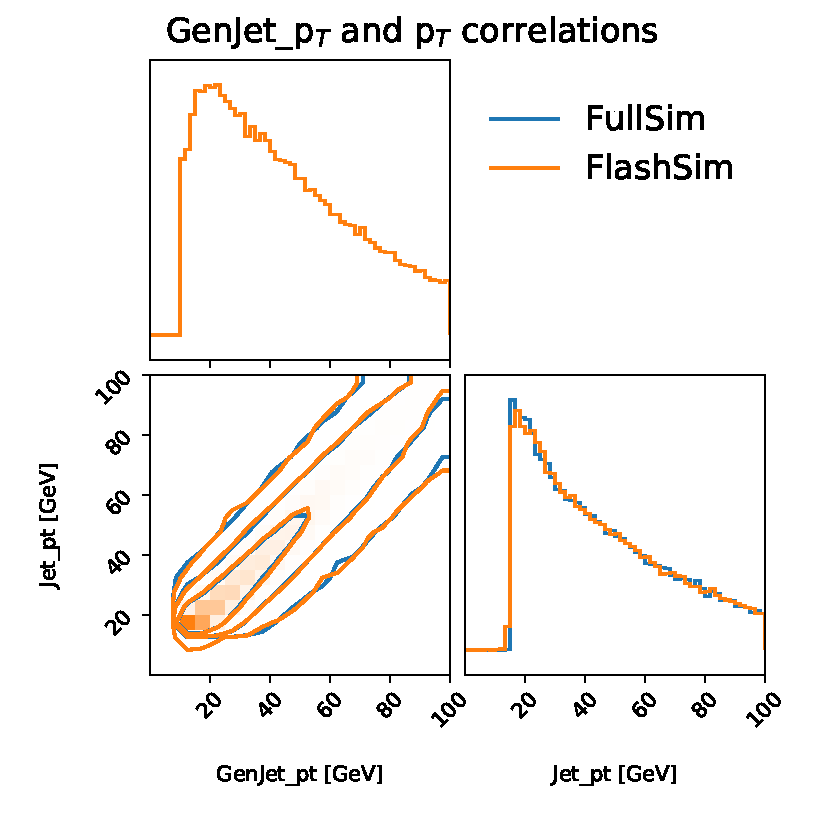
\includegraphics[width=0.45\linewidth]{gfx/ch5/corrjet4.pdf}}
    \subfloat[]
    { 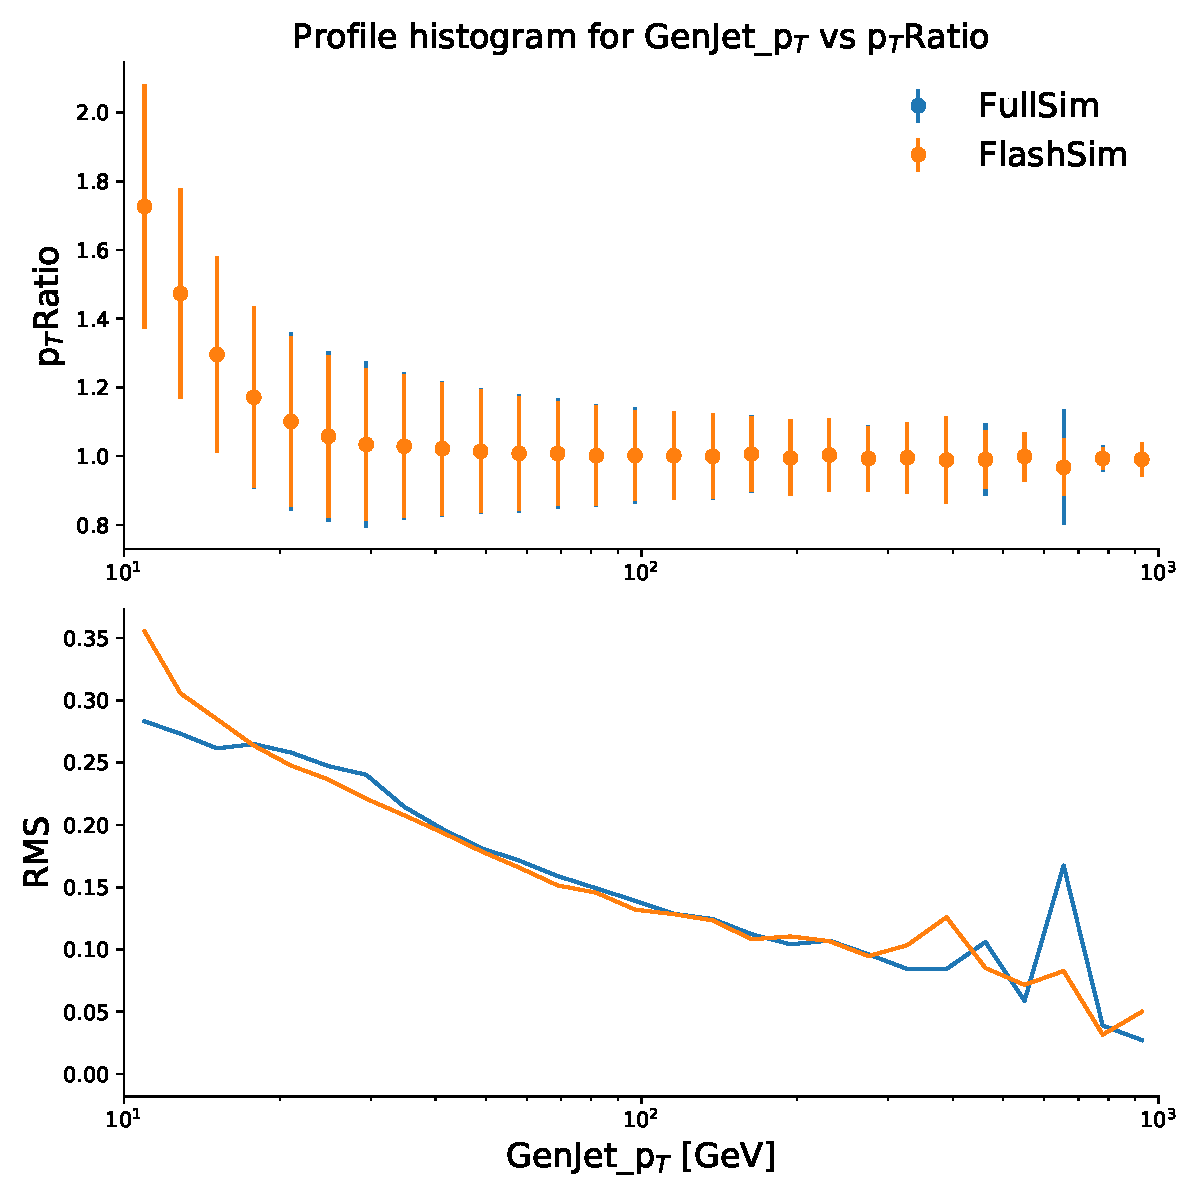
\includegraphics[width=0.45\linewidth]{gfx/ch5/profhist.pdf}} 
    \caption[Conditioning]{ (a) As we would expect the Gen-p$_T$ is crucial in determining the final-state p$_T$. Higher Gen-values correspond to higher reco-values. (b) Not only does the p$_T$Ratio decrease as the GenJet p$_T$ increases (highly energetic jets have a reconstructed p$_T$ closer to the Gen-value), but the RMS correctly decreases as well because of constant error terms being divided by larger Gen-values.}\label{fig:condit}
    
\end{figure}

Additionally, because the \texttt{partonFlavour} conditioning variable allow us to specify the quark content of a jet, we can study how related quantities depend on this input. As a key example, we study the behaviour of the \texttt{btagDeepB} b-tagging distribution as we vary the parton input for the jet generation. Figure \ref{fig:roc1} shows how the distribution changes according to the ground truth value specified as input: as expected, jets being conditioned with a b content present higher values of b-tagging, with a sharp peak at one, while those coming from u, d, s are clearly peaked aroun smaller values. Now we could think of defining a threshold and assign a reconstructed b content to all those jets higher than that value. We would naturally mistag some events, leading us to define a \emph{flase-positive} ratio and a \emph{true-positive} one. A standard figure of merit for these cases is the \emph{Receiving operating characteristic} curve, which plots the TPR against the FPR for all possible threshold choices. Figure \ref{fig:roc1} shows it for our model in log scale, showing minimal deviations from the target FullSim curve.


\begin{figure}
    \myfloatalign
    \subfloat[]
    {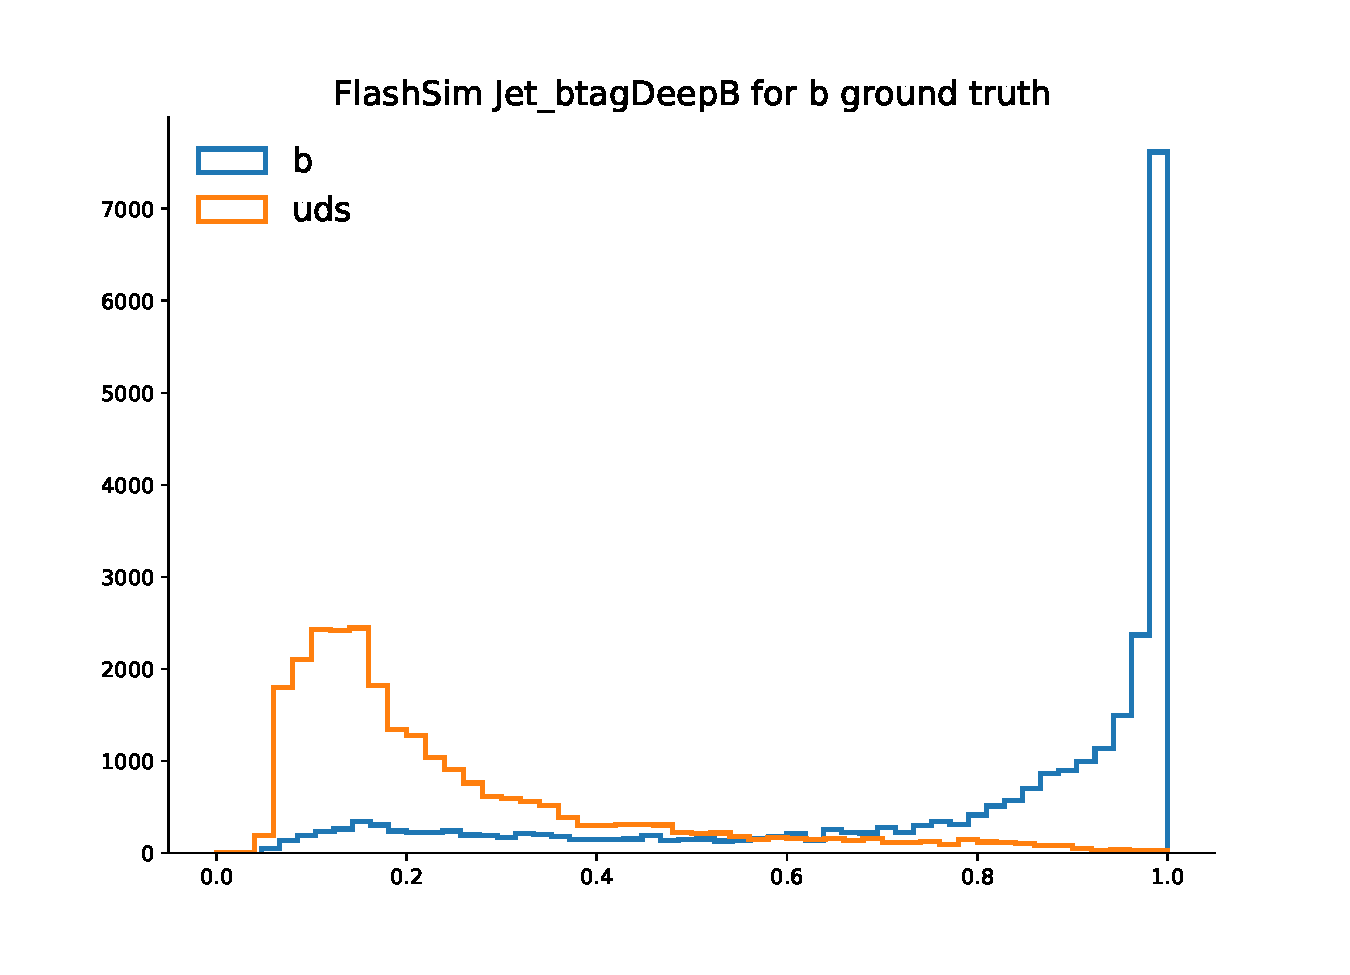
\includegraphics[width=0.45\linewidth]{gfx/ch5/btagj.pdf}}
    \subfloat[]
    { 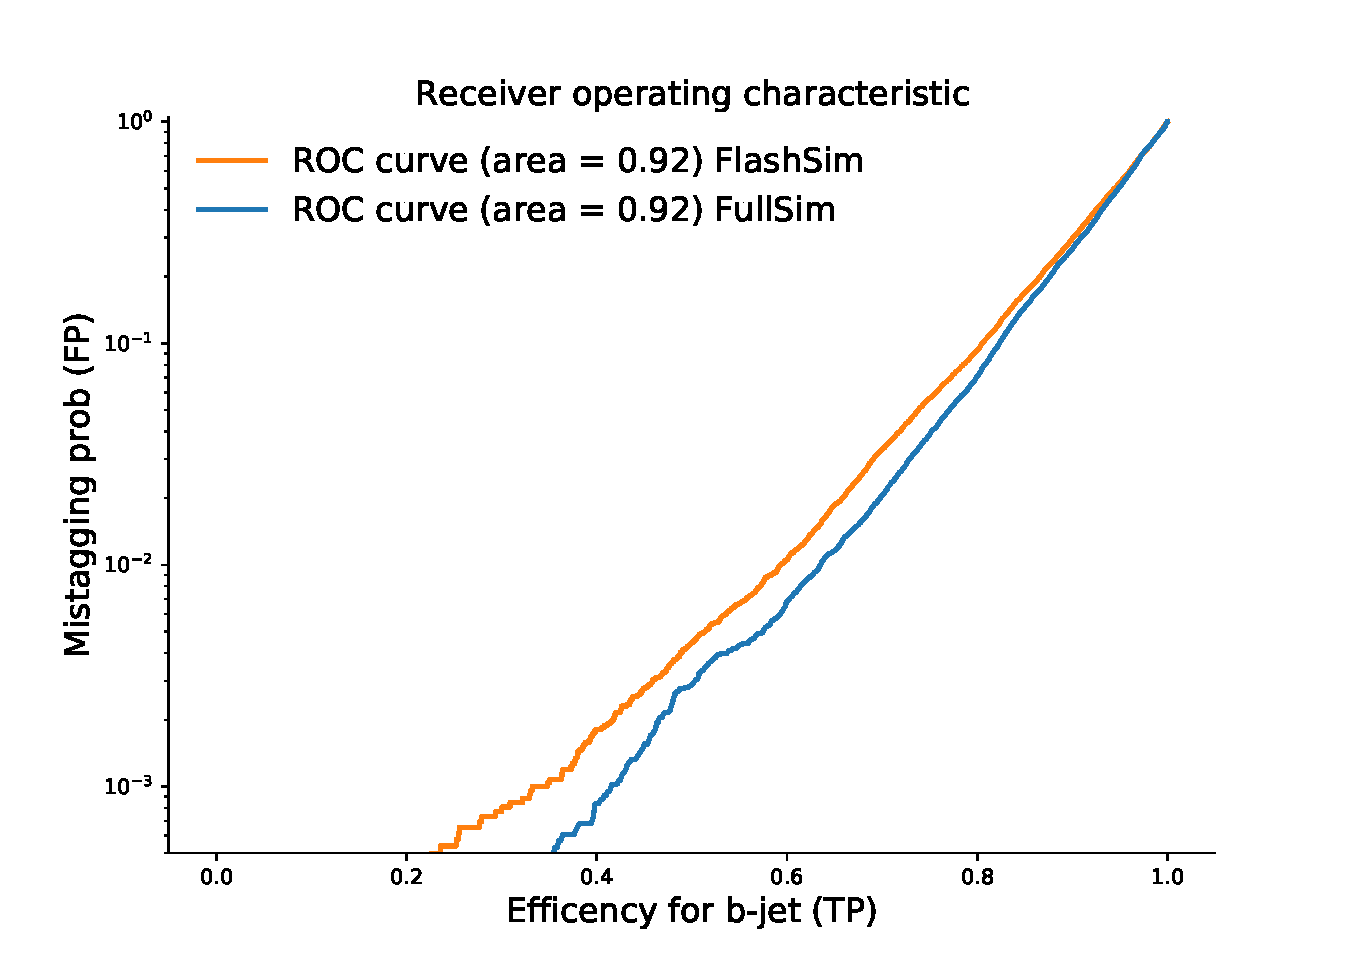
\includegraphics[width=0.45\linewidth]{gfx/ch5/roc.pdf}} 
    \caption[b-tagging and ROC]{ (a) The b-tagging distribution shape correctly depends upon the specified quark content at the Gen-level. (b) The ROC curve for the FlashSim approaches that for FullSim, showing that even on derived quantities our approach is capable of delivering satisfying results.}\label{fig:roc1}
    
\end{figure}

Because our results are not as close to FullSim as before, we would like to compare them with other competing approaches to asses the goodness of our own methodology. In order to do so, for a previous, simpler iteration of the jets model which was presented in the CMS Machine learning Forum of April 2022, we compared the ROC curves between FullSim, FastSim and FlashSim on a $10^{6}$ samples set (not previously seen during training). Results are shown in Figure \ref{fig:allrocs} shows the comparison. We can see that while the ROC between our approach and FullSim is actually indistiguishable for TPR higher than 0.8, the FastSim ROC completely \emph{overshoots} the target, due to oversimplifications in the simulation approach. With longer training times and additional loss terms addressing this type of conditioning, we are confident that the performance of FlashSim could be improved even more.

\begin{figure}
    \centering
    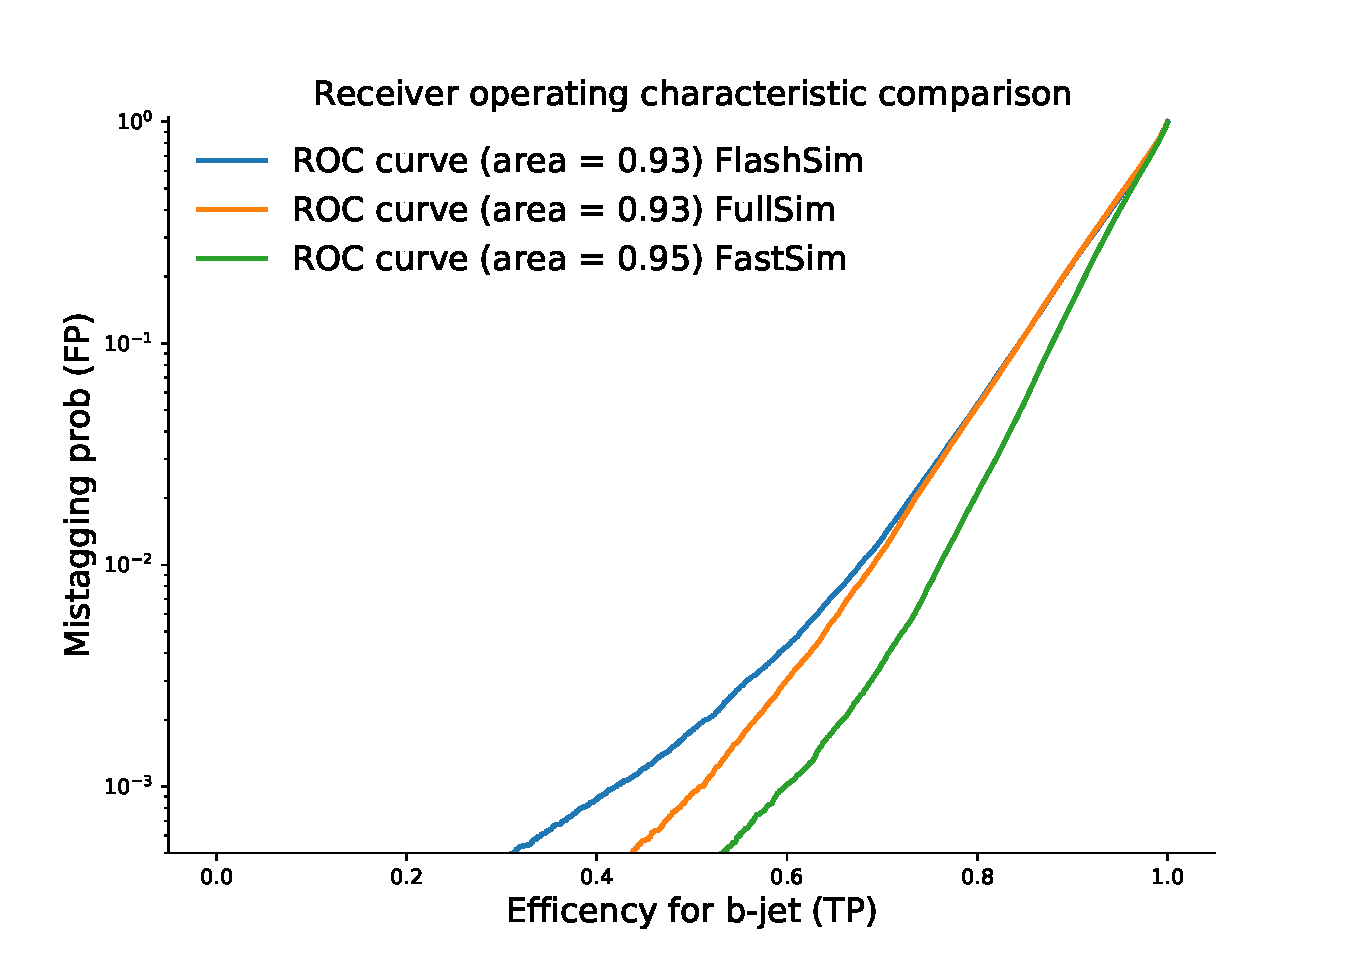
\includegraphics[width=\linewidth]{gfx/ch5/allrocs.pdf}
    \caption[ROC Comparison]{The FlashSim ROC can actually obtain close results to FullSim, while FastSim fails to replicate the target ROC.}
    \label{fig:allrocs}
\end{figure}


\subsection{Speed}

A crucial result obtained is the \emph{generation speed}: for both jets and muons we managed to generate samples in batches of $10^{4}$ in $\approx$ 0.3 seconds each, corresponding to a generation speed of raw samples of about 33,300 \emph{samples per second} (33 kHz) \emph{meaning a six orders of magnitude speedup when compared to FullSim}! Even considering possible reduction due to preprocessing and data loading, this result testify to the potential of the current methodology to completely redefine our approach to event simulation, at least at the NanoAOD level.

What is more, the $10^{4}$ batch size for generation was limited only by the VRAM of the GPU being used, meaning that more powerful GPUs, ideally working in parallel, could achieve even faster generation times.


\section{A prototype end-to-end analysis sample generator}\label{sec:progen}

We conclude by presenting the general idea for an end-to-end analysis sample generator in the NanoAOD format. The key concept can be easily grasped through Figure \ref{fig:endtoend}: a FullSim NanoAOD file gets processed and its Gen-level values extracted for eventual preprocessing. Then, the values are passed to the two networks, which generate raw samples which are finally postprocessed to reobtaine physical distributions and combined into a single, NanoAOD-like file format. The whole process can be executed by a single call to a \texttt{Python} script, which leverages the \texttt{ROOT C} interpreter for running the extraction and the \texttt{uproot} package for structuring and saving the data directly in the \texttt{.root} format, in a corresponding \texttt{TTree} data structure.

\begin{figure}
    \centering
    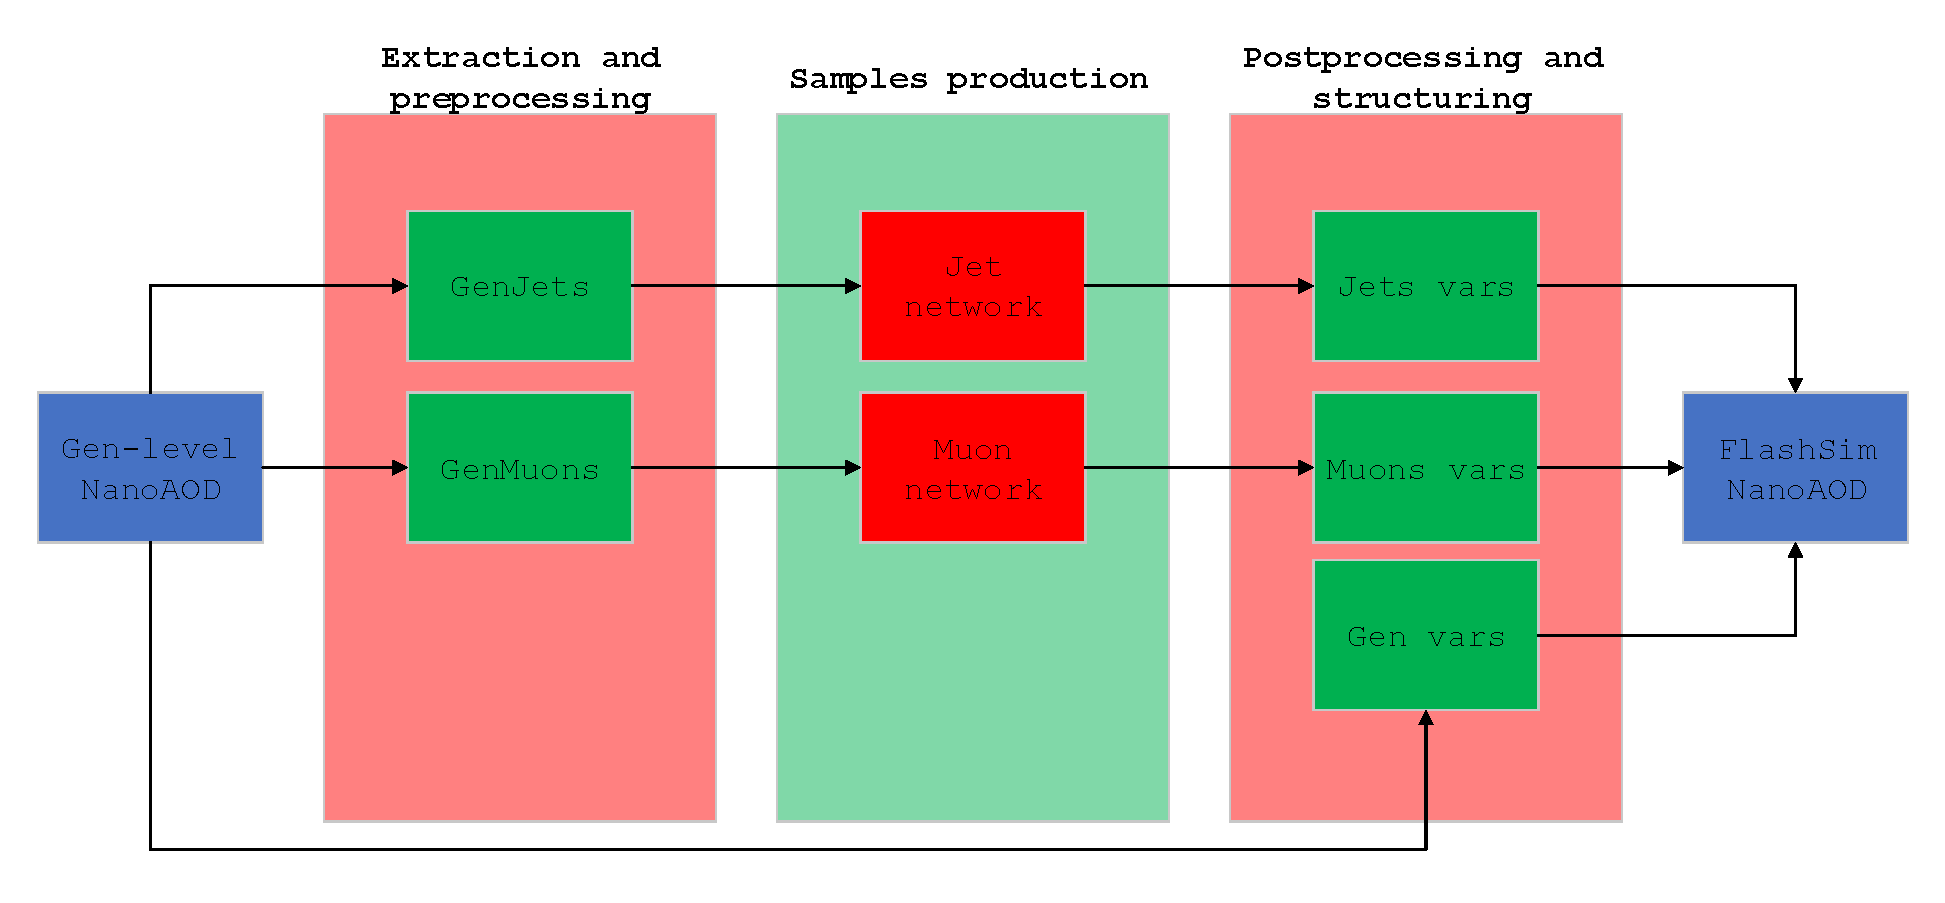
\includegraphics[width=\linewidth]{gfx/ch5/endtoend.pdf}
    \caption[end-toend sample generator]{The basic steps behind the prototype for an end-to-end sample generator.}
    \label{fig:endtoend}
\end{figure}

This prototype has been tested on the full \emph{TTJets} dataset (t$\overline{\text{t}}$ process) for the H$\rightarrow\mu^+\mu^-$ study of \cite{CMS-PAS-HIG-19-006}. What is more, we actually extended the use of the generator to \emph{different physical processes}: \emph{Drell-Yan}, \emph{Electroweak} and two \emph{Signal (H)} datasets were processed as well and stored for the comparison of the next chapter. The two signal datasets differ in the theoretical technique employed for \emph{systematic inclusion of higher order QCD effects}: one employed the \texttt{POWHEG} method \cite{Nason_2004}, the other the \texttt{MadGraph5\_aMC@NLO} \cite{powpow} one.
In total we processed more than 200 files, meaning several millions of events, in less than one day.

In the end, we proved that our networks can be integrated into the existing software base and can be used for obtaining files in the exact same standard of that used in current analysis at CMS. We were able to asses two major characteristics of our approach:

\begin{outline}
    \1 The NF networks are actually capable of tackling other processes, inherently different from the training one: both distributions and correlations maintain good accord with FullSim samples, despite considerable changes from the training set. This is a crucial property if we are to move away from the prototyping stage to a more realistic, full-scale and general-purpose NanoAOD simulator;
    \1 Considering the whole preprocessing/postprocessing/disk writing overhead, the whole process took about 440 second or 7 minutes on the typical NanoAOD file of the TTJets dataset (about $10^{6}$ events per file), once again testyfing to the speed of the current methodology.
\end{outline}